\chapter{Virtual Topologies for \texorpdfstring{\MPI/}{MPI} Processes}
\mpitermtitleindex{topologies}
\label{sec:topol}
\label{chap:topol}

\section{Introduction}

This chapter discusses the \MPI/ \mpiterm{virtual topology} mechanism.  A \mpitermni{virtual topology} is an extra,
optional attribute that one can give to an intra-communicator; \mpitermni{virtual topologies}
cannot be added to inter-communicators.  A \mpitermni{virtual topology} can provide a convenient
naming mechanism for the \MPI/ processes of a group (within a communicator), and
additionally, may assist the runtime system in mapping the processes onto
hardware.

As stated in Chapter~\ref{chap:context},
a group in \MPI/ is an ordered set of \mpicode{n} process identifiers (henceforth
\MPI/ processes). Each \MPI/ process in
the group is assigned a rank between \mpicode{0} and \mpicode{n-1}. In many parallel
applications, a linear assignment of integer ranks to the \MPI/ processes does not adequately reflect the logical
communication pattern of the \MPI/ processes (which is usually determined by the
underlying problem geometry and the numerical algorithm used).  Often the
\MPI/ processes are arranged in topological patterns such as two- or
three-dimensional grids. More generally, the logical \MPI/ process arrangement is
described by a graph.  In this chapter we will refer to this logical \MPI/ process
arrangement as the \mpitermni{virtual topology}\mpitermindex{topology!virtual}\mpitermindex{virtual topology}.

A clear distinction must be made between the \mpitermni{virtual topology} and the
topology of the underlying, physical hardware.  The \mpitermni{virtual topology} can be
exploited by the system in the assignment of processes to physical processors,
if this helps to improve the communication performance on a given machine. How
this mapping is done, however, is outside the scope of \MPI/.  The description
of the \mpitermni{virtual topology}, on the other hand, depends only on the application,
and is machine-independent. 
The functions that are described in this chapter
deal with machine-independent 
mapping and communication on \mpitermni{virtual topologies}.

\begin{rationale}
Though physical mapping is not discussed, the
existence of the \mpitermni{virtual topology} information may be used as advice by
the runtime system.
There are well-known techniques for mapping grid/torus structures to
hardware topologies such as hypercubes or grids. For more
complicated graph structures good heuristics often yield nearly optimal
results \cite{suprenum}. On the other hand,
if there is no way for the user to specify the logical process
arrangement as a \mpitermni{virtual topology}, a random mapping is most
likely to result. On some machines, this will lead to
unnecessary contention in the interconnection network.
Some details about predicted and measured
performance improvements that result from good process-to-processor
mapping on wormhole-routing architectures can be found in
\cite{wormhole2,wormhole1}.

Besides possible performance benefits, the \mpitermni{virtual topology} can
function as a convenient, process-naming structure, with 
significant
benefits for program readability and notational power in
message-passing programming.
\end{rationale}

\section{Virtual Topologies}
\mpitermtitleindexsubmain{virtual}{topology}
The communication pattern of a set of \MPI/ processes can be represented by a
graph. The nodes 
represent \MPI/ processes,
and the edges connect \MPI/ processes that
communicate with each other. \MPI/ provides message-passing between any pair
of \MPI/ processes in a group. There is no requirement for opening a channel
explicitly. Therefore, a ``missing link'' in the user-defined graph of \MPI/ processes
does not prevent the corresponding \MPI/ processes from exchanging messages. It
means rather that this connection is neglected in the \mpitermni{virtual topology}. This
strategy implies
that the \mpitermni{virtual topology} gives no convenient way of naming this pathway of
communication.  Another possible consequence is that an automatic mapping tool
(if one exists for the runtime environment) will not take account of this edge
when mapping.  

Specifying the \mpitermni{virtual topology}
in terms of a graph is sufficient for all applications. However, in
many applications the graph structure is regular, and the detailed set-up
of the graph would be inconvenient for the user and might be less
efficient at
run time. A large fraction of all parallel applications use \MPI/ process topologies
like rings, two- or higher-dimensional grids, or tori. These structures are
completely defined by the number of dimensions and the numbers of \MPI/ processes in
each coordinate direction.  Also, the mapping of grids and tori is generally
an easier problem than that of general graphs.  Thus, it is desirable to
address these cases explicitly.

The coordinates of \MPI/ processes in a Cartesian structure begin their numbering at $0$.
Row-major numbering is always used for the \MPI/ processes in a
Cartesian structure. This means that, for example, for four \MPI/ processes in a
\mpicode{$(2 \times 2)$} grid, the relationship between their ranks in the group
and their coordinates in the \mpitermni{virtual topology} is as follows:
\begin{center}
\begin{tabular}{ll}
 coord (0,0): & rank 0 \\
 coord (0,1): & rank 1 \\
 coord (1,0): & rank 2 \\
 coord (1,1): & rank 3 \\
\end{tabular}
\end{center}

\section{Embedding in \texorpdfstring{\MPI/}{MPI}}
The support for \mpitermni{virtual topologies} as defined in this chapter is
consistent with other parts of \MPI/, and, whenever possible,
makes use of functions that are defined elsewhere.
Topology information is associated with communicators. It is added
to communicators using the caching mechanism described in
Chapter~\ref{chap:context}.

Information representing a \mpitermni{virtual topology} may be added to a communicator at the time of its creation.
If a communicator creation function adds information representing a \mpitermni{virtual topology} to the output communicator it creates, then it either propagates the topology representation from the input communicator to the output communicator, or adds a new topology representation generated from the input parameters that describe a \mpitermni{virtual topology}.
The description of every \MPI/ communicator creation function explicitly states how topology information is handled.
Communicator creation functions that create new topology representations are described in \sectionref{subsec:topol-construct}.


\section{Overview of the Functions}
\label{subsec:topol-overview}

\MPI/ supports three types of \mpitermni{virtual topology}:
\mpitermdefni{Cartesian}\mpitermdefindex{Cartesian!topology}\mpitermdefindex{topology!Cartesian},
\mpitermdefni{graph}\mpitermdefindex{graph!topology}\mpitermdefindex{topology!graph}, and
\mpitermdefni{distributed graph}\mpitermdefindex{distributed graph!topology}\mpitermdefindex{topology!distributed graph}.  
The function \mpifunc{MPI\_CART\_CREATE}
can be used to create Cartesian topologies, the function
\mpifunc{MPI\_GRAPH\_CREATE} can be used to create graph topologies, and the
functions \mpifunc{MPI\_DIST\_GRAPH\_CREATE\_ADJACENT} and
\mpifunc{MPI\_DIST\_GRAPH\_CREATE} can be used to create distributed graph
topologies.
These topology creation functions are collective.  As with
other collective calls, the program must be written to work correctly,
whether the call synchronizes or not.

The above topology creation functions take as input an existing communicator
\mpiarg{comm\_old},
which defines the set of \MPI/ processes on which the topology is to be
mapped.
For \mpifunc{MPI\_GRAPH\_CREATE} and \mpifunc{MPI\_CART\_CREATE},
all input arguments must have identical
values on all \MPI/ processes of the group of \mpiarg{comm\_old}.
When calling \mpifunc{MPI\_GRAPH\_CREATE}, each \MPI/ process specifies all
nodes and edges in the graph. In contrast, the functions
\mpifunc{MPI\_DIST\_GRAPH\_CREATE\_ADJACENT} or
\mpifunc{MPI\_DIST\_GRAPH\_CREATE} are used to
specify the graph in a distributed fashion, whereby each \MPI/ process only
specifies a subset of the edges in the graph such that the entire graph
structure is defined collectively across the set of \MPI/ processes.
Therefore the \MPI/ processes provide different values for the
arguments specifying the graph. However, all \MPI/ processes must give the
same value for \mpiarg{reorder} and the \mpiarg{info} argument. In all cases, a
new communicator \mpiarg{comm\_topol} is created that
carries the topological structure as cached information (see
Chapter~\ref{chap:context}). In analogy to function
\mpifunc{MPI\_COMM\_CREATE}, no cached information propagates from
\mpiarg{comm\_old} to \mpiarg{comm\_topol}.

\mpifunc{MPI\_CART\_CREATE} can be used to describe Cartesian structures of
arbitrary dimension. For each coordinate direction one specifies whether the
\MPI/ process structure is periodic or not.
Note that an $n$-dimensional hypercube is
an $n$-dimensional torus with two processes per coordinate direction. Thus,
special support for hypercube structures is not necessary.  The local
auxiliary function \mpifunc{MPI\_DIMS\_CREATE} can be used to compute a balanced
distribution of \MPI/ processes among a given number of dimensions.

%%% WDG: Do we really need this rationale - it is over 20 years old now.
% htor: agreed, removed as ticket-0 change
%\begin{rationale}Similar functions are contained in
%EXPRESS \cite{express} and PARMACS.  \end{rationale}

\MPI/ defines functions to query a communicator for topology information.
The function \mpifunc{MPI\_TOPO\_TEST} is used to query for the type of topology
associated with a communicator. Depending on the topology type,
different information can be extracted. For a graph topology, the
functions \mpifunc{MPI\_GRAPHDIMS\_GET} and \mpifunc{MPI\_GRAPH\_GET} retrieve the graph topology information
that is associated with the communicator. Additionally, the
functions \mpifunc{MPI\_GRAPH\_NEIGHBORS\_COUNT} and
\mpifunc{MPI\_GRAPH\_NEIGHBORS} can be used
to obtain the neighbors of an arbitrary node in the graph. For a
distributed graph topology, the functions
\mpifunc{MPI\_DIST\_GRAPH\_NEIGHBORS\_COUNT}
and \mpifunc{MPI\_DIST\_GRAPH\_NEIGHBORS} can be used to obtain the neighbors of the
calling \MPI/ process. For a Cartesian topology, the function
\mpifunc{MPI\_CARTDIM\_GET} returns the number of dimensions and \mpifunc{MPI\_CART\_GET} returns the numbers of
\MPI/ processes in each dimension and periodicity of the associated Cartesian topology. Additionally, the functions
\mpifunc{MPI\_CART\_RANK} and \mpifunc{MPI\_CART\_COORDS} translate Cartesian coordinates into a group rank, and
vice-versa. The function \mpifunc{MPI\_CART\_SHIFT} provides the information needed
to communicate with neighbors along a Cartesian dimension. All of these
query functions are local.

For Cartesian topologies, the function
\mpifunc{MPI\_CART\_SUB} can be used to extract a Cartesian subspace
(analogous to \mpifunc{MPI\_COMM\_SPLIT}). This function is collective
over the input communicator's group.

The two additional functions, \mpifunc{MPI\_GRAPH\_MAP} and
\mpifunc{MPI\_CART\_MAP}, are, in general, not called by the user directly. However,
together with the communicator manipulation functions presented in
Chapter~\ref{chap:context}, they are sufficient to implement all other
topology functions.  Section~\ref{subsec:topol-lowlevel} outlines such
an implementation.
 
The neighborhood collective communication routines
\mpifunc{MPI\_NEIGHBOR\_ALLGATHER}, \mpifunc{MPI\_NEIGHBOR\_ALLGATHERV}, 
\mpifunc{MPI\_NEIGHBOR\_ALLTOALL},\flushline % fix for margins
\mpifunc{MPI\_NEIGHBOR\_ALLTOALLV},
and \mpifunc{MPI\_NEIGHBOR\_ALLTOALLW}
communicate with the nearest neighbors on the topology associated with
the communicator.
The nonblocking variants are
\mpifunc{MPI\_INEIGHBOR\_ALLGATHER}, \mpifunc{MPI\_INEIGHBOR\_ALLGATHERV}, 
\mpifunc{MPI\_INEIGHBOR\_ALLTOALL}, \mpifunc{MPI\_INEIGHBOR\_ALLTOALLV},
and \mpifunc{MPI\_INEIGHBOR\_ALLTOALLW}.

\section{Topology Constructors}
\label{subsec:topol-construct}

\subsection{Cartesian Constructor}
\mpitermtitleindex{Cartesian!topology}
\mpitermtitleindex{topology!Cartesian}
\label{subsec:topol-cartesian-constructor}

\begin{mpi-binding}
    function_name("MPI_Cart_create")
    
    parameter("comm_old", "COMMUNICATOR", desc=r"input communicator")
    parameter(
        "ndims", "NUM_DIMS", desc=r"number of dimensions of Cartesian grid"
    )
    parameter(
        "dims",
        "DIMENSION",
        length="ndims",
        constant=True,
        desc=(
            r"integer array of size \mpiarg{ndims} specifying the number of "
            r"processes in each dimension"
        ),
        suppress="lis_paren",
    )
    parameter(
        "periods",
        "LOGICAL",
        length="ndims",
        constant=True,
        desc=(
            r"logical array of size \mpiarg{ndims} specifying whether the "
            r"grid is periodic (\mpicode{true}) or not (\mpicode{false}) in "
            r"each dimension"
        ),
        suppress="lis_paren",
    )
    parameter(
        "reorder",
        "LOGICAL",
        desc=r"ranks may be reordered (\mpicode{true}) or not (\mpicode{false})",
    )
    parameter(
        "comm_cart",
        "COMMUNICATOR",
        direction="out",
        desc=r"new communicator with associated Cartesian topology",
    )
\end{mpi-binding}

\mpifunc{MPI\_CART\_CREATE} returns a handle to a new communicator to which the
Cartesian topology information is attached.  If \mpiarg{reorder}\mpicode{ = false} then
the rank of each \MPI/ process in the group of the new communicator is identical
to its rank in the group of the old communicator.  If \mpiarg{reorder}\mpicode{ = true}
then the procedure may reorder the ranks of the \MPI/ processes (possibly so as to
choose a good embedding of the \mpitermni{virtual topology} onto the physical machine).
If the total size of the Cartesian grid is smaller than the size of the group
of \mpiarg{comm\_old}, then some \MPI/ processes return \mpiconst{MPI\_COMM\_NULL}, in
analogy to \mpifunc{MPI\_COMM\_SPLIT}.
If \mpiarg{ndims} is zero then a zero-dimensional Cartesian topology is created. The
call is erroneous if it specifies a grid that is larger than the group size or if
\mpiarg{ndims} is negative.
\mpifunc{MPI\_CART\_CREATE} will associate information representing a Cartesian topology
with the specified number of dimensions, numbers of \MPI/ processes in each coordinate
direction, and periodicity with the new communicator.

\subsection{Cartesian Convenience Function: \texorpdfstring{\mpifunc{MPI\_DIMS\_CREATE}}{MPI\_DIMS\_CREATE}}

For Cartesian topologies, the function \mpifunc{MPI\_DIMS\_CREATE} helps the user
select a balanced distribution of \MPI/ processes per coordinate direction,
depending on the number of \MPI/ processes in the group to be balanced and optional
constraints that can be specified by the user.

\begin{mpi-binding}
    function_name("MPI_Dims_create")
    
    # this is a count of nodes
    parameter("nnodes", "COMM_SIZE", desc=r"number of nodes in a grid")
    parameter("ndims", "NUM_DIMS", desc=r"number of Cartesian dimensions")
    parameter(
        "dims",
        "DIMENSION",
        length="ndims",
        direction="inout",
        desc=(
            r"integer array of size \mpiarg{ndims} specifying the number of "
            r"nodes in each dimension"
        ),
        suppress="lis_paren",
    )
\end{mpi-binding}

The entries in the array \mpiarg{dims} are set to describe a Cartesian grid
with \mpiarg{ndims} dimensions and a total of \mpiarg{nnodes} nodes.  The
dimensions are set to be as close to each other as possible, using an
appropriate divisibility algorithm.  The caller may
further constrain the operation of this routine by specifying elements
of array \mpicode{dims}. If \mpicode{dims[i]} is set to a positive number, the
routine will not modify the number of nodes in dimension \mpicode{i};
only those entries where \mpicode{dims[i]}\mpicode{ = 0} are modified by the call.

Negative input values of \mpicode{dims[i]} are erroneous.
An error will occur if \mpicode{nnodes} is not a multiple of
$$\prod_{i, \textsf{\scriptsize{}dims}[i]\neq 0} \mpicode{dims[$i$]}.$$ %%ALLOWLATEX% - because mpicode does not properly work in formula subscripts

For \mpicode{dims[i]} set by the call, \mpicode{dims[i]} will be ordered in
nonincreasing order.  Array \mpicode{dims} is suitable for use as input to
routine \mpifunc{MPI\_CART\_CREATE}.  \mpifunc{MPI\_DIMS\_CREATE} is local.
If \mpiarg{ndims} is zero and \mpiarg{nnodes} is one, \mpifunc{MPI\_DIMS\_CREATE} returns \error{MPI\_SUCCESS}.

\begin{example}
\label{topol-exA}
The use of the array argument \mpicode{dims} in \mpifunc{MPI\_DIMS\_CREATE}.
\Exindex{Neutral}{Dims create}{MPI\_DIMS\_CREATE}%

\begin{center}
\begin{tabular}{|l|l|l|}
\hline
\mpicode{dims} & function call & \mpicode{dims} \\
before call &              & on return \\
\hline
(0,0)      & \mpifunc{MPI\_DIMS\_CREATE}\code{(6, 2, dims)} & (3,2) \\
(0,0)      & \mpifunc{MPI\_DIMS\_CREATE}\code{(7, 2, dims)} & (7,1) \\
(0,3,0)    & \mpifunc{MPI\_DIMS\_CREATE}\code{(6, 3, dims)} & (2,3,1) \\
(0,3,0)    & \mpifunc{MPI\_DIMS\_CREATE}\code{(7, 3, dims)} & erroneous call \\
\hline
\end{tabular}
\end{center}
\end{example}

\subsection{Graph Constructor}
\mpitermtitleindex{graph!topology}
\mpitermtitleindex{topology!graph}
\label{subsec:topol-graph-constructor}

\begin{mpi-binding}
    function_name("MPI_Graph_create")
    
    parameter("comm_old", "COMMUNICATOR", desc=r"input communicator")
    parameter("nnodes", "COMM_SIZE", desc=r"number of nodes in graph")
    parameter(
        "index",
        "INDEX",
        length="nnodes",
        constant=True,
        desc=r"array of integers describing node degrees (see below)",
        suppress="lis_paren",
    )
    parameter(
        "edges",
        "RANK",
        length="*",
        constant=True,
        desc=r"array of integers describing graph edges (see below)",
        suppress="lis_paren",
    )
    parameter(
        "reorder",
        "LOGICAL",
        desc=r"ranks may be reordered (\mpicode{true}) or not (\mpicode{false})",
    )
    parameter(
        "comm_graph",
        "COMMUNICATOR",
        direction="out",
        desc=r"new communicator with associated graph topology",
    )
\end{mpi-binding}

\mpifunc{MPI\_GRAPH\_CREATE} returns a handle to a new communicator to which the
graph topology information is attached.  If \mpiarg{reorder}\mpicode{ = false} then the
rank of each \MPI/ process in the group of the new communicator is identical to its rank in the
group of the old communicator.  If \mpiarg{reorder}\mpicode{ = true} then the procedure may 
reorder the ranks of the \MPI/ processes.  If the number of nodes in the graph
(\mpiarg{nnodes}) is smaller than the size of the group of
\mpiarg{comm\_old}, then \mpiconst{MPI\_COMM\_NULL} is returned by some \MPI/ processes, in
analogy to \mpifunc{MPI\_CART\_CREATE} and \mpifunc{MPI\_COMM\_SPLIT}.
If the graph is empty, i.e., \mpiarg{nnodes}\mpicode{ = 0},
then \mpiconst{MPI\_COMM\_NULL} is returned in all \MPI/ processes. 
The call
is erroneous if it specifies a graph that is larger than the group size of the
input communicator.

The three parameters \mpiarg{nnodes}, \mpiarg{index} and \mpiarg{edges} define the graph
structure.
\mpiarg{nnodes} is the number of nodes of the graph.   The nodes are numbered
from \mpicode{0} to \mpicode{nnodes-1}.
The 
\mpicode{i}-th 
entry of array \mpiarg{index} stores the total number of
neighbors of the first \mpicode{i} graph nodes.   The lists of neighbors of
nodes \mpicode{0, 1, \ldots, nnodes-1} are stored in consecutive locations in array
\mpiarg{edges}.  The array \mpiarg{edges} is a flattened representation
of the edge lists.
The total number of entries in \mpiarg{index} is \mpiarg{nnodes} and
the total number of entries in \mpiarg{edges} is equal to the number of
graph edges.

The definitions of the arguments \mpicode{nnodes}, \mpicode{index}, and
\mpicode{edges} are illustrated with the following simple example.

\begin{example}
\label{topol-exB}
\Exindex{Neutral}{Graph create}{MPI\_GRAPH\_CREATE}%
Specification of the adjacency matrix for \mpifunc{MPI\_GRAPH\_CREATE}.

Assume there are four \MPI/ processes with ranks 0, 1, 2, 3 in the input communicator with the following
adjacency matrix:

\begin{center}
\begin{tabular}{|c|l|}
\hline
\MPI/ process & neighbors \\
\hline
0       & 1, 3      \\
1       & 0         \\
2       & 3         \\
3       & 0, 2      \\
\hline
\end{tabular}
\end{center}
\noindent Then, the input arguments are:

\begin{center}
\begin{tabular}{ll}
nnodes = & 4 \\
index = & 2, 3, 4, 6 \\
edges = & 1, 3, 0, 3, 0, 2
\end{tabular}
\end{center}

Thus, in C, \code{index[0]} is the degree of node zero, and \code{index[i] -
index[i-1]} is the degree of node \code{i, i=1, \ldots, nnodes-1};
the list of neighbors of node zero is stored in \code{edges[j]}, for
$\code{0} \leq \code{j} \leq \code{index[0]}-\code{1}$ and the 
list of neighbors of node \code{i},
$\code{i} > \code{0}$,
is stored in \code{edges[j]}, $\code{index[i-1]} \leq \code{j} \leq 
\code{index[i]}-\code{1}$.

In Fortran, \code{index(1)} is the degree of node zero, and \code{index(i+1) -
index(i)} is the degree of node \code{i, i=1, \ldots, nnodes-1};
the list of neighbors of node zero is stored in \code{edges(j)}, for
$\code{1} \leq \code{j} \leq \code{index(1)}$ and the list of neighbors of node
\code{i}, $\code{i} > \code{0}$,
is stored in \code{edges(j)}, $\code{index(i)+1} \leq \code{j} \leq 
\code{index(i+1)}$.

\end{example}

A single \MPI/ process is allowed to be defined multiple times in the list of
neighbors of an \MPI/ process (i.e., there may be multiple edges between two
\MPI/ processes). An \MPI/ process is also allowed to be a neighbor to itself (i.e., a self
loop in the graph). The adjacency matrix is allowed to be nonsymmetric.
\begin{users}
Performance implications of using multiple edges or a nonsymmetric
adjacency matrix are not defined. The definition of a node-neighbor
edge does not imply a direction of the communication.
\end{users} 

\begin{implementors}
The following topology information is likely to be stored with a communicator:
\begin{itemize}
\item Type of topology (Cartesian/graph)
\item For a Cartesian topology:
   \begin{enumerate}
   \item \mpicode{ndims} (number of dimensions)
   \item \mpicode{dims} (numbers of \MPI/ processes per coordinate direction)
   \item \mpicode{periods} (periodicity information)
   \item \mpicode{own\_position} (own position in grid, could also be computed
                          from rank and dims)
   \end{enumerate}
\item For a graph topology:
   \begin{enumerate}
   \item \mpicode{index}
   \item \mpicode{edges}
   \end{enumerate}
which are the arrays defining the graph structure.
\end{itemize}

For a graph structure the number of nodes is equal to the number of \MPI/ processes
in the group. Therefore, the number of nodes does not have to be stored explicitly.  An
additional zero entry at the start of array \mpiarg{index} simplifies
access to the topology information.
\end{implementors}

\subsection{Distributed Graph Constructor}
\mpitermtitleindex{distributed graph!topology}
\mpitermtitleindex{topology!distributed graph}
\label{subsec:topol-distgraph-constructor} % Sect. 7.5.3a p.247

\mpifunc{MPI\_GRAPH\_CREATE} requires that each \MPI/ process passes the
full (global) communication graph to the call. This limits the
scalability of this constructor. With the distributed graph interface,
the communication graph is specified in a fully distributed
fashion. Each \MPI/ process specifies only the part of the communication
graph of which it is aware. Typically, this could be the set of
\MPI/ processes from which the \MPI/ process will eventually receive or get data,
or the set of \MPI/ processes to which the \MPI/ process will send or put data, or
some combination of such edges.  Two different interfaces can be used
to create a distributed graph
topology. \mpifunc{MPI\_DIST\_GRAPH\_CREATE\_ADJACENT} creates a
distributed graph communicator with each \MPI/ process specifying each of its
incoming and outgoing (adjacent) edges in the logical communication
graph and thus requires minimal communication during
creation. \mpifunc{MPI\_DIST\_GRAPH\_CREATE}
provides full flexibility such that any \MPI/ process can indicate that
communication will occur between any pair of \MPI/ processes in the graph.

To provide better possibilities for optimization by the \MPI/ library,
the distributed graph constructors permit weighted communication edges
and take an \mpiarg{info} argument that can further influence process
reordering or other optimizations performed by the \MPI/ library. For
example, hints can be provided on how edge weights are to be
interpreted, the quality of the reordering, and/or the time permitted
for the \MPI/ library to process the graph.

\begin{mpi-binding}
    function_name("MPI_Dist_graph_create_adjacent")
    
    parameter("comm_old", "COMMUNICATOR", desc=r"input communicator")
    parameter(
        "indegree",
        "DEGREE",
        desc=r"size of \mpiarg{sources} and \mpiarg{sourceweights} arrays",
    )
    parameter(
        "sources",
        "RANK_NNI",
        length="indegree",
        constant=True,
        desc=(
            r"ranks of \MPI/ processes for which the calling process is a "
            r"destination"
        ),
    )
    parameter(
        "sourceweights",
        "WEIGHT",
        length="*",
        constant=True,
        desc=r"weights of the edges into the calling \MPI/ process",
    )
    parameter(
        "outdegree",
        "DEGREE",
        desc=r"size of \mpiarg{destinations} and \mpiarg{destweights} arrays",
    )
    parameter(
        "destinations",
        "RANK_NNI",
        length="outdegree",
        constant=True,
        desc=r"ranks of \MPI/ processes for which the calling \MPI/ process is a source",
    )
    parameter(
        "destweights",
        "WEIGHT",
        length="*",
        constant=True,
        desc=r"weights of the edges out of the calling \MPI/ process",
    )
    parameter(
        "info",
        "INFO",
        desc=r"hints on optimization and interpretation of weights",
    )
    parameter(
        "reorder",
        "LOGICAL",
        desc=(
            r"ranks may be reordered (\mpicode{true}) or "
            r"not~(\mbox{\mpicode{false}})"
        ),
    )
    parameter(
        "comm_dist_graph",
        "COMMUNICATOR",
        direction="OUT",
        desc=r"new communicator with associated distributed graph topology",
    )
\end{mpi-binding}

\mpifunc{MPI\_DIST\_GRAPH\_CREATE\_ADJACENT} returns a handle to a new
communicator to which the distributed graph topology information is
attached.  Each \MPI/ process passes all information about its incoming and
outgoing edges in the virtual distributed graph topology.  The calling
\MPI/ processes must ensure that each edge of the graph is described in the
source and in the destination process with the same weights. If there
are multiple edges for a given (\mpiarg{source},\mpiarg{dest}) pair, then the sequence
of the weights of these edges does not matter. The complete
communication topology is the combination of all edges shown in the
\mpiarg{sources} arrays of all \MPI/ processes in \mpiarg{comm\_old}, which must be
identical to the combination of all edges shown in the
\mpiarg{destinations} arrays.  Source and destination \MPI/ processes must be
specified by their rank in the group of 
\mpiarg{comm\_old}. This allows a fully distributed
specification of the communication graph.  Isolated \MPI/ processes (i.e.,
\MPI/ processes with no outgoing or incoming edges, that is, \MPI/ processes that
have specified \mpiarg{indegree} and \mpiarg{outdegree} as zero and
thus do not occur as source or destination in the graph
specification) are allowed.

The call creates a new communicator \mpiarg{comm\_dist\_graph} of
distributed graph topology type to which topology information has been
attached. The number of \MPI/ processes in \mpiarg{comm\_dist\_graph} is
identical to the number of \MPI/ processes in \mpiarg{comm\_old}. The call to
\mpifunc{MPI\_DIST\_GRAPH\_CREATE\_ADJACENT} is collective.

Weights are specified as nonnegative integers and can be used to
influence the process mapping strategy and other internal \MPI/
optimizations. For instance, approximate count arguments of later
communication calls along specific edges could be used as their edge
weights. Multiplicity of edges can likewise indicate more intense
communication between pairs of \MPI/ processes. However, the exact meaning
of edge weights is not specified by the \MPI/ standard and is left to
the implementation. In C or Fortran, an application can supply the
special value \mpiconstmain{MPI\_UNWEIGHTED} for the weight array to indicate
that all edges have the same (effectively no) weight. It is erroneous to supply
\mpiconst{MPI\_UNWEIGHTED} for some but not all \MPI/ processes of
\mpiarg{comm\_old}. 
If the graph is weighted but
\mpiarg{indegree} or \mpiarg{outdegree} is zero, then \mpiconstmain{MPI\_WEIGHTS\_EMPTY} or any
arbitrary array may be passed to \mpiarg{sourceweights} or
\mpiarg{destweights} respectively. Note that \mpiconst{MPI\_UNWEIGHTED} and
\mpiconst{MPI\_WEIGHTS\_EMPTY} are not special weight values; rather they
are special values for the total array argument.  In Fortran,
\mpiconst{MPI\_UNWEIGHTED} and \mpiconst{MPI\_WEIGHTS\_EMPTY} are objects like
\mpiconst{MPI\_BOTTOM} (not usable for initialization or assignment).
See Section~\ref{subsec:named-constants}. % Subsection 2.5.4.

\begin{users}
In the case of an empty weights array argument passed while constructing
a weighted graph, one should not pass \code{NULL} because the value of
\mpiconst{MPI\_UNWEIGHTED} may be equal to \code{NULL}. The value of this argument
would then be indistinguishable from \mpiconst{MPI\_UNWEIGHTED} to the
implementation. In this case \mpiconst{MPI\_WEIGHTS\_EMPTY} should be used
instead.
\end{users}

\begin{implementors}
It is recommended that \mpiconst{MPI\_UNWEIGHTED} not be implemented as
\code{NULL}.
\end{implementors}

\begin{rationale}
To ensure backward compatibility, \mpiconst{MPI\_UNWEIGHTED} may still be
implemented as \code{NULL}. See \annexref{subsec:22to30}.
\end{rationale}

The meaning of the \mpiarg{info} and \mpiarg{reorder} arguments is defined
in the description of the following routine.

\begin{mpi-binding}
    function_name("MPI_Dist_graph_create")
    
    parameter("comm_old", "COMMUNICATOR", desc=r"input communicator")
    parameter(
        "n",
        "ARRAY_LENGTH_NNI",
        desc=r"number of source nodes for which this \MPI/ process specifies edges",
    )
    parameter(
        "sources",
        "RANK_NNI",
        constant=True,
        length="n",
        desc=(
            r"array containing the \mpiarg{n} source nodes for "
            r"which this \MPI/ process specifies edges"
        ),
    )
    parameter(
        "degrees",
        "DEGREE",
        length="n",
        constant=True,
        desc=(
            r"array specifying the number of destinations for each source "
            r"node in the source node array"
        ),
    )
    parameter(
        "destinations",
        "RANK_NNI",
        length="*",
        constant=True,
        desc=r"destination nodes for the source nodes in the source node array",
    )
    parameter(
        "weights",
        "WEIGHT",
        length="*",
        constant=True,
        desc=r"weights for source to destination edges",
    )
    parameter(
        "info",
        "INFO",
        desc=r"hints on optimization and interpretation of weights",
    )
    parameter(
        "reorder",
        "LOGICAL",
        desc=(
            r"ranks may be reordered (\mpicode{true}) or "
            r"not~(\mbox{\mpicode{false}})"
        ),
    )
    parameter(
        "comm_dist_graph",
        "COMMUNICATOR",
        direction="OUT",
        desc=r"new communicator with associated distributed graph topology",
    )
\end{mpi-binding}

\mpifunc{MPI\_DIST\_GRAPH\_CREATE} returns a handle to a new
communicator to which the distributed graph topology information is
attached. Concretely, each \MPI/ process calls the constructor with a set of
directed (\mpiarg{source},\mpiarg{destination}) communication edges as
described below. Every \MPI/ process passes an array of \mpiarg{n} source
nodes in the \mpiarg{sources} array.  For each source node, a
nonnegative number of destination nodes is specified in the
\mpiarg{degrees} array. The destination nodes are stored in the
corresponding consecutive segment of the \mpiarg{destinations}
array. More precisely, if the \mpiarg{i}-th node in \mpiarg{sources} is
\mpiarg{s}, this specifies \mpiarg{degrees[i]} edges \mpiarg{(s,d)}
with \mpiarg{d} of the \mpiarg{j}-th such edge stored in
\mpiarg{destinations[degrees[0]+$\ldots$+degrees[i-1]+j]}. The weight of
this edge is stored in
\mpiarg{weights[degrees[0]+$\ldots$+degrees[i-1]+j]}.  Both the
\mpiarg{sources} and the \mpiarg{destinations} arrays may contain the
same node more than once, and the order in which nodes are listed as
destinations or sources is not significant. Similarly, different
processes may specify edges with the same source and destination
nodes. Source and destination nodes must be
specified by their rank in the group of \mpiarg{comm\_old}.
Different \MPI/ processes may specify different numbers
of source and destination nodes, as well as different source to
destination edges.  This allows a fully distributed specification of
the communication graph.  Isolated \MPI/ processes (i.e., \MPI/ processes with no
outgoing or incoming edges, that is, \MPI/ processes that do not occur as
source or destination node in the graph specification) are allowed.

The call creates a new communicator \mpiarg{comm\_dist\_graph} of
distributed graph topology type to which topology information has been
attached. The number of \MPI/ processes in \mpiarg{comm\_dist\_graph} is
identical to the number of \MPI/ processes in \mpiarg{comm\_old}. The call to
\mpifunc{MPI\_DIST\_GRAPH\_CREATE} is collective.

If \mpiarg{reorder}\mpicode{ = false}, all \MPI/ processes will have the same rank in
\mpiarg{comm\_dist\_graph} as in \mpiarg{comm\_old}. If
\mpiarg{reorder}\mpicode{ = true} then the \MPI/ library is free to remap to
other \MPI/ processes (of \mpiarg{comm\_old}) in order to improve
communication on the edges of the communication graph. The weight
associated with each edge is a hint to the \MPI/ library about the
amount or intensity of communication on that edge, and may be used to
compute a ``best'' reordering.

Weights are specified as nonnegative integers and can be used to
influence the \MPI/ process remapping strategy and other internal \MPI/
optimizations. For instance, approximate count arguments of later
communication calls along specific edges could be used as their edge
weights. Multiplicity of edges can likewise indicate more intense
communication between pairs of \MPI/ processes. However, the exact meaning
of edge weights and multiplicity of edges is not specified by the \MPI/ standard and is left to
the implementation. In C or Fortran, an application can supply the
special value \mpiconst{MPI\_UNWEIGHTED} for the weight array to indicate
that all edges have the same (effectively no) weight. It is erroneous to supply \mpiconst{MPI\_UNWEIGHTED} for some but not all \MPI/ processes of
\mpiarg{comm\_old}. 
If the graph is weighted but \mpiarg{n}\mpicode{ = 0}, then
\mpiconst{MPI\_WEIGHTS\_EMPTY} or any arbitrary array may be passed to
weights. Note that \mpiconst{MPI\_UNWEIGHTED} and
\mpiconst{MPI\_WEIGHTS\_EMPTY} are not special weight values; rather
they are special values for the total array argument. In Fortran,
\mpiconst{MPI\_UNWEIGHTED} and \mpiconst{MPI\_WEIGHTS\_EMPTY} are objects like
\mpiconst{MPI\_BOTTOM} (not usable for initialization or assignment).
See Section~\ref{subsec:named-constants}. % Subsection 2.5.4.

\begin{users}
In the case of an empty weights array argument passed while constructing
a weighted graph, one should not pass \code{NULL} because the value of
\mpiconst{MPI\_UNWEIGHTED} may be equal to \code{NULL}. The value of this argument
would then be indistinguishable from \mpiconst{MPI\_UNWEIGHTED} to the
implementation. \mpiconst{MPI\_WEIGHTS\_EMPTY} should be used
instead.
\end{users}

\begin{implementors}
It is recommended that \mpiconst{MPI\_UNWEIGHTED} not be implemented as
\code{NULL}.
\end{implementors}

\begin{rationale}
To ensure backward compatibility, \mpiconst{MPI\_UNWEIGHTED} may still be
implemented as \code{NULL}. See \annexref{subsec:22to30}.
\end{rationale}

The meaning of the \mpiarg{weights} argument can be influenced by the
\mpiarg{info} argument. The info argument can be used to guide the
mapping of \MPI/ processes to the hardware; possible options include minimizing the maximum number of
edges between processes on different SMP nodes, or minimizing the sum
of all such edges.  As described in \sectionref{subsec:info}, 
an \MPI/ implementation is not obliged to follow
specific hints, and it is valid for an \MPI/ implementation not to do
any reordering.  An \MPI/ implementation may specify more \mpiarg{info}
(\mpiarg{key},\mpiarg{value}) pairs. All \MPI/ processes must specify the same set of (\mpiarg{key},\mpiarg{value})
\mpiarg{info} pairs.

\begin{implementors}
\MPI/ implementations must document every additionally supported (\mpiarg{key},\mpiarg{value})
\mpiarg{info} pair. \mpiconst{MPI\_INFO\_NULL} is always valid, and may
indicate the default creation of the distributed graph topology to the
\MPI/ library.

An implementation does not explicitly need to construct the topology
from its distributed parts. However, all \MPI/ processes can construct the
full topology from the distributed specification and use this in a
call to \mpifunc{MPI\_GRAPH\_CREATE} to create the topology.  This may serve
as a reference implementation of the functionality, and may be
acceptable for small communicators. However, a scalable high-quality
implementation would save the topology graph in a distributed way.
\end{implementors}

\begin{example}
\label{topol-exG}
\Exindex{Neutral}{Dist graph creation}{MPI\_DIST\_GRAPH\_CREATE,MPI\_DIST\_GRAPH\_CREATE\_ADJACENT}%
Several ways to specify the adjacency matrix for \mpifunc{MPI\_DIST\_GRAPH\_CREATE} and \mpifunc{MPI\_DIST\_GRAPH\_CREATE\_ADJACENT}.

As for Example~\ref{topol-exB},
assume there are four \MPI/ processes with ranks 0, 1, 2, 3 in the input communicator with the following adjacency matrix and
unit edge weights:
%
\begin{center}
\begin{tabular}{|c|l|}
\hline
\MPI/ process & neighbors \\
\hline
0       & 1, 3      \\
1       & 0         \\
2       & 3         \\
3       & 0, 2      \\
\hline
\end{tabular}
\end{center}
With \mpifunc{MPI\_DIST\_GRAPH\_CREATE}, this graph could be
constructed in many different ways. One way would be that each \MPI/ process
specifies its outgoing edges. The arguments per \MPI/ process would be:
%
\begin{center}
\begin{tabular}{|c|l|l|l|l|l|}
\hline
\MPI/ process &  \mpiarg{n}  & \mpiarg{sources} & \mpiarg{degrees} & 
\mpiarg{destinations} & \mpiarg{weights} \\
\hline
0       &  1  & 0       & 2       & 1,3          & 1,1     \\
1       &  1  & 1       & 1       & 0            & 1       \\
2       &  1  & 2       & 1       & 3            & 1       \\
3       &  1  & 3       & 2       & 0,2          & 1,1     \\
\hline
\end{tabular}
\end{center}

Another way would be to pass the whole graph on \MPI/ process with rank \code{0} in the input communicator, which could be
done with the following arguments per \MPI/ process:
%
\begin{center}
\begin{tabular}{|c|l|l|l|l|l|}
\hline
\MPI/ process &  \mpiarg{n}  & \mpiarg{sources} & \mpiarg{degrees} & 
\mpiarg{destinations} & \mpiarg{weights}     \\
\hline
0       &  4  & 0,1,2,3 & 2,1,1,2 & 1,3,0,3,0,2  & 1,1,1,1,1,1 \\
1       &  0  & -       & -       & -            & -           \\
2       &  0  & -       & -       & -            & -           \\
3       &  0  & -       & -       & -            &             \\
\hline
\end{tabular}
\end{center}

In both cases above, the application could supply \mpiconst{MPI\_UNWEIGHTED}
instead of explicitly providing identical weights.

\mpifunc{MPI\_DIST\_GRAPH\_CREATE\_ADJACENT} could be used to specify
this graph using the following arguments:
%
\begin{center}
\begin{tabular}{|c|l|l|l|l|l|l|}
\hline
\MPI/ process &  \mpiarg{indegree}  & \mpiarg{sources} & \mpiarg{sourceweights} & 
\mpiarg{outdegree}   & \mpiarg{destinations} & \mpiarg{destweights}    \\
\hline
0       &  2         & 1,3     & 1,1           & 2           & 1,3          & 1,1            \\
1       &  1         & 0       & 1             & 1           & 0            & 1              \\
2       &  1         & 3       & 1             & 1           & 3            & 1              \\
3       &  2         & 0,2     & 1,1           & 2           & 0,2          & 1,1            \\
\hline
\end{tabular}
\end{center}
\end{example}

\begin{example}
\label{topol-exH}
\Exindex{C}{Dist\_graph\_create}{MPI\_Dist\_graph\_create}%
Cartesian grid plus diagonals specified with \mpifunc{MPI\_DIST\_GRAPH\_CREATE}.

A two-dimensional $P \times Q$ torus where all \MPI/ processes communicate along the
dimensions and along the diagonal edges cannot be modeled with
Cartesian topologies, but can easily be captured with
\mpifunc{MPI\_DIST\_GRAPH\_CREATE} as shown in the following code. In this
example, the communication along the dimensions is twice as heavy as
the communication along the diagonals:

%%HEADER
%%LANG: C
%%FRAGMENT
%%DECL: int P, Q;
%%ENDHEADER
\begin{lstlisting}[language={[MPI]C}]
/*
Input:     dimensions P, Q
Condition: number of MPI processes equal to P*Q
*/
int rank, x, y;
int sources[1], degrees[1];
int destinations[8], weights[8];
MPI_Comm comm_dist_graph;

MPI_Comm_rank(MPI_COMM_WORLD, &rank);

/* get x and y dimension */
y=rank/P; x=rank%P;

/* get my communication partners along x dimension */
destinations[0] = P*y+(x+1)%P; weights[0] = 2;
destinations[1] = P*y+(P+x-1)%P; weights[1] = 2;

/* get my communication partners along y dimension */
destinations[2] = P*((y+1)%Q)+x; weights[2] = 2;
destinations[3] = P*((Q+y-1)%Q)+x; weights[3] = 2;

/* get my communication partners along diagonals */
destinations[4] = P*((y+1)%Q)+(x+1)%P; weights[4] = 1;
destinations[5] = P*((Q+y-1)%Q)+(x+1)%P; weights[5] = 1;
destinations[6] = P*((y+1)%Q)+(P+x-1)%P; weights[6] = 1;
destinations[7] = P*((Q+y-1)%Q)+(P+x-1)%P; weights[7] = 1;

sources[0] = rank;
degrees[0] = 8;
MPI_Dist_graph_create(MPI_COMM_WORLD, 1, sources, degrees, destinations,
                      weights, MPI_INFO_NULL, 1, &comm_dist_graph);
\end{lstlisting}
\end{example}

\subsection{Topology Inquiry Functions}
\label{subsec:topol-inquiry}

If a \mpitermni{virtual topology} has been defined with one of the above functions, then the topology
information can be looked up using inquiry functions. They all are local
calls.

\begin{mpi-binding}
    function_name("MPI_Topo_test")
    
    parameter("comm", "COMMUNICATOR", desc=r"communicator")
    parameter(
        "status",
        "TOPOLOGY_TYPE",
        direction="OUT",
        desc=r"topology type of communicator \mpiarg{comm}",
    )
\end{mpi-binding}

The function \mpifunc{MPI\_TOPO\_TEST} returns the type of topology that
is associated with a communicator.

The output value \mpiarg{status} is one of the following:
\begin{constlist}
\constmainitem {MPI\_GRAPH}{graph topology}
\constmainitem {MPI\_CART}{Cartesian topology}
\constmainitem {MPI\_DIST\_GRAPH}{distributed graph topology}
\constitem {MPI\_UNDEFINED}{no topology}
\end{constlist}

\begin{mpi-binding}
    function_name("MPI_Graphdims_get")
    
    parameter(
        "comm",
        "COMMUNICATOR",
        desc=r"communicator with associated graph topology",
    )
    parameter(
        "nnodes",
        "ARRAY_LENGTH",
        direction="OUT",
        desc=(
            r"number of nodes in graph (same as number of \MPI/ processes in the "
            r"group of \mpiarg{comm})"
        ),
    )
    parameter(
        "nedges",
        "ARRAY_LENGTH",
        direction="OUT",
        desc=r"number of edges in graph",
    )
\end{mpi-binding}
\begin{sloppy}
The functions \mpifunc{MPI\_GRAPHDIMS\_GET} and
\mpifunc{MPI\_GRAPH\_GET} retrieve the graph \mbox{topology} information
that is associated with the communicator.
The information provided by \mpifunc{MPI\_GRAPHDIMS\_GET} can be used
to dimension the
vectors \mpiarg{index} and \mpiarg{edges} correctly for the following call
to \mpifunc{MPI\_GRAPH\_GET}.
\end{sloppy}

\begin{mpi-binding}
    function_name("MPI_Graph_get")

    parameter("comm", "COMMUNICATOR", desc=r"communicator with associated graph topology")
    parameter(
        "maxindex",
        "ARRAY_LENGTH",
        desc=r"length of vector \mpiarg{index} in the calling program",
    )
    parameter(
        "maxedges",
        "ARRAY_LENGTH",
        desc=r"length of vector \mpiarg{edges} in the calling program",
    )
    parameter(
        "index",
        "INDEX",
        length="maxindex",
        direction="OUT",
        desc=(
            r"array of integers containing the graph structure (for details "
            r"see the definition of \mpifunc{MPI_GRAPH_CREATE})"
        ),
        suppress="lis_paren",
    )
    parameter(
        "edges",
        "RANK",
        length="maxedges",
        direction="OUT",
        desc=r"array of integers containing the graph structure",
        suppress="lis_paren",
    )
\end{mpi-binding}

\begin{mpi-binding}
    function_name("MPI_Cartdim_get")
    
    parameter(
        "comm", "COMMUNICATOR", desc=r"communicator with associated Cartesian topology"
    )
    parameter(
        "ndims",
        "NUM_DIMS",
        direction="out",
        desc=r"number of dimensions of the Cartesian structure",
    )
\end{mpi-binding}

The functions \mpifunc{MPI\_CARTDIM\_GET} and
\mpifunc{MPI\_CART\_GET} return the Cartesian topology information that is
associated with the communicator.
If \mpiarg{comm} is associated with a zero-dimensional Cartesian topology,
\mpifunc{MPI\_CARTDIM\_GET} returns \mpiarg{ndims}\mpicode{ = 0} and \mpifunc{MPI\_CART\_GET} will keep
all output arguments unchanged. 

\begin{mpi-binding}
    function_name("MPI_Cart_get")
    
    parameter(
        "comm", "COMMUNICATOR", desc=r"communicator with associated Cartesian topology"
    )
    parameter(
        "maxdims",
        "ARRAY_LENGTH",
        desc=(
            r"length of vectors \mpiarg{dims}, \mpiarg{periods}, and "
            r"\mpiarg{coords} in the calling program"
        ),
    )
    parameter(
        "dims",
        "DIMENSION",
        direction="out",
        length="maxdims",
        desc=r"number of \MPI/ processes for each Cartesian dimension",
    )
    parameter(
        "periods",
        "LOGICAL",
        direction="out",
        length="maxdims",
        desc=(
            r"periodicity (\mpicode{true}/\mpicode{false}) for each Cartesian "
            r"dimension"
        ),
    )
    parameter(
        "coords",
        "COORDINATE",
        direction="out",
        length="maxdims",
        desc=r"coordinates of calling \MPI/ process in Cartesian structure",
    )
\end{mpi-binding}
If \mpiarg{maxdims} in a call to \mpifunc{MPI\_CART\_GET} is less than the number of dimensions of the Cartesian topology associated with the communicator \mpiarg{comm}, the outcome is unspecified.

\begin{mpi-binding}
    function_name("MPI_Cart_rank")
    
    parameter(
        "comm", "COMMUNICATOR", desc=r"communicator with associated Cartesian topology"
    )
    parameter(
        "coords",
        "COORDINATE",
        length="*",
        constant=True,
        desc=(
            r"integer array (of size \mpiarg{ndims}) specifying the "
            r"Cartesian coordinates of an \MPI/ process"
        ),
        suppress="lis_paren",
    )
    parameter("rank", "RANK", direction="out", desc=r"rank of specified \MPI/ process within group of \mpiarg{comm}")
\end{mpi-binding}

For a communicator with an associated Cartesian topology, the function
\mpifunc{MPI\_CART\_RANK} translates the logical coordinates of an \MPI/ process to
the corresponding rank in the group of the communicator.
For dimension \mpicode{i} with \mpicode{periods(i) = true}, if the coordinate,
\mpicode{coords(i)}, is out of range, that is, \mbox{\mpicode{coords(i) $<$ 0}} or
\mbox{\mpicode{coords(i) $\geq$ dims(i)}}, it is shifted back to the interval
\mbox{\mpicode{0 $\leq$ coords(i) $<$ dims(i)}} automatically. Out-of-range
coordinates are erroneous for nonperiodic dimensions.
 
If \mpiarg{comm} is associated with a zero-dimensional Cartesian topology,
\mpishortarg{coords} is not significant and 0 is returned in \mpiarg{rank}. 

\begin{mpi-binding}
    function_name("MPI_Cart_coords")
    
    parameter(
        "comm", "COMMUNICATOR", desc=r"communicator with associated Cartesian topology"
    )
    parameter(
        "rank", "RANK", desc=r"rank of an \MPI/ process within group of \mpiarg{comm}"
    )
    parameter(
        "maxdims",
        "ARRAY_LENGTH",
        desc=r"length of vector  \mpiarg{coords} in the calling program",
    )
    
    # JMS MPI-3.1 erroneously stated "...of size ndims..."
    # RR ndims in MPI-1.1 to 3.1 was correct; change to maxdims in MPI-4.0 was wrong;
    # RR in MPI-4.1 corrected by wording that is analog to spec in MPI_CART_GET
    parameter(
        "coords",
        "COORDINATE",
        length="maxdims",
        direction="out",
        desc=(
            r"coordinates of the \MPI/ process with the rank \mpiarg{rank} in Cartesian structure"
        ),
    )
\end{mpi-binding}

The inverse mapping, rank-to-coordinates translation is provided by
\mpifunc{MPI\_CART\_COORDS}.
If \mpiarg{comm} is associated with a zero-dimensional Cartesian topology,
\mpiarg{coords} will be unchanged. 
If \mpiarg{maxdims} is less than the number of dimensions of the Cartesian topology associated with the communicator \mpiarg{comm}, the outcome is unspecified.

\begin{mpi-binding}
    function_name("MPI_Graph_neighbors_count")
    
    parameter("comm", "COMMUNICATOR", desc=r"communicator with associated graph topology")
    parameter("rank", "RANK", desc=r"rank of \MPI/ process in group of \mpiarg{comm}")
    parameter(
        "nneighbors",
        "ARRAY_LENGTH",
        direction="out",
        desc=r"number of neighbors of specified \MPI/ process",
    )
\end{mpi-binding}

\begin{mpi-binding}
    function_name("MPI_Graph_neighbors")

    parameter("comm", "COMMUNICATOR", desc=r"communicator with associated graph topology")
    parameter("rank", "RANK", desc=r"rank of \MPI/ process in group of \mpiarg{comm}")
    parameter(
        "maxneighbors", "ARRAY_LENGTH", desc=r"size of array \mpiarg{neighbors}"
    )
    parameter(
        "neighbors",
        "RANK",
        direction="out",
        length="maxneighbors",
        desc=r"ranks of \MPI/ processes that are neighbors to specified \MPI/ process",
    )
\end{mpi-binding}

\begin{sloppy}
\mpifunc{MPI\_GRAPH\_NEIGHBORS\_COUNT} and \mpifunc{MPI\_GRAPH\_NEIGHBORS} provide  
adjacency information for a graph topology.  
The returned count and array of neighbors for the queried rank will 
both include \emph{all} neighbors and reflect the same edge ordering as 
was specified by the original call to \mpifunc{MPI\_GRAPH\_CREATE}. 
Specifically, \mpifunc{MPI\_GRAPH\_NEIGHBORS\_COUNT} and 
\mpifunc{MPI\_GRAPH\_NEIGHBORS} will return values based on the original 
\mpicode{index} and \mpicode{edges} array passed to \mpifunc{MPI\_GRAPH\_CREATE}
(for the purpose of this example, we assume that \mpicode{index[-1]} is zero):

\end{sloppy}
\begin{itemize} 
\item The number of neighbors (\mpiarg{nneighbors}) returned from\flushline % fix for margins
  \mpifunc{MPI\_GRAPH\_NEIGHBORS\_COUNT} will be (\mpicode{index[rank]} - 
  \mpicode{index[rank-1]}). 
\item The \mpiarg{neighbors} array returned from 
  \mpifunc{MPI\_GRAPH\_NEIGHBORS} will be {\gb\mbox{\mpicode{edges[index[rank-1]]}}}
  through {\gb\mbox{\mpicode{edges[index[rank]-1]}}}.
\end{itemize} 
 
\begin{example}
  \label{topol-graph-neighbors-count} 
\Exindex{Neutral}{Graph creation and neighbors count}{MPI\_GRAPH\_NEIGHBORS\_COUNT,MPI\_GRAPH\_NEIGHBORS,MPI\_GRAPH\_CREATE}%
Inquiry of graph topology information.

  Assume there are four \MPI/ processes with ranks 0, 1, 2, 3 in the input communicator with the following
  adjacency matrix (note that some neighbors are listed multiple times):

\begin{center}
  \begin{tabular}{|c|l|} 
  \hline 
  \MPI/ process & neighbors \\ 
  \hline 
  0       & 1, 1, 3   \\ 
  1       & 0, 0      \\ 
  2       & 3         \\ 
  3       & 0, 2, 2   \\ 
  \hline 
  \end{tabular} 
\end{center}
   
Thus, the input arguments to \mpifunc{MPI\_GRAPH\_CREATE} are:
  % 
\begin{center}
  \begin{tabular}{ll} 
  nnodes = & 4 \\ 
  index = & 3, 5, 6, 9 \\ 
  edges = & 1, 1, 3, 0, 0, 3, 0, 2, 2 
  \end{tabular} 
\end{center}   

\noindent Therefore, calling \mpifunc{MPI\_GRAPH\_NEIGHBORS\_COUNT} and
  \mpifunc{MPI\_GRAPH\_NEIGHBORS} for each of the four \MPI/ processes will return:

\begin{center}
  \begin{tabular}{ccl} 
  \multicolumn{1}{c}{\textbf{Input rank}} & \multicolumn{1}{c}{\textbf{Count}} & 
  \multicolumn{1}{c}{\textbf{Neighbors}} \\ 
  \hline 
  0 & 3 & 1, 1, 3 \\ 
  1 & 2 & 0, 0 \\ 
  2 & 1 & 3 \\ 
  3 & 3 & 0, 2, 2 \\ 
  \hline 
  \end{tabular}
\end{center}
\end{example} 

\begin{example}
\label{topol-exC}
\Exindex{Neutral}{Graph creation}{MPI\_GRAPH\_CREATE}%
Using a communicator with an associated graph topology that represents a shuffle-exchange network.

Suppose that \mpicode{comm} is a communicator with a
shuffle-exchange topology.   The group has $2^n$ members.
Each \MPI/ process is labeled by $a_1 , \ldots, a_n$ with $a_i \in
\{0,1\}$, and has three neighbors:
exchange($a_1 , \ldots, a_n ) = a_1 ,\ldots, a_{n-1}, \bar{a}_n$
($\bar{a} =
1-a$), shuffle($a_1 , \ldots, a_n )= a_2 , \ldots,
a_{n}, a_1$, and unshuffle($a_1 , \ldots, a_n ) = a_n , a_1 , \ldots , a_{n-1}$.
The graph adjacency list is illustrated below for $n=3$.

\begin{center}
\begin{tabular}{|cc|ccc|}
\hline
\multicolumn{2}{|c|}{\textbf{node}}&{\textbf{exchange}}&{\textbf{shuffle}}&{\textbf{unshuffle}}\\
  &       & neighbors(1) & neighbors(2) & neighbors(3) \\
\hline
0 & (000) & 1 & 0 & 0\\
1 & (001) & 0 & 2 & 4\\
2 & (010) & 3 & 4 & 1\\
3 & (011) & 2 & 6 & 5\\
4 & (100) & 5 & 1 & 2\\
5 & (101) & 4 & 3 & 6\\
6 & (110) & 7 & 5 & 3\\
7 & (111) & 6 & 7 & 7\\
\hline
\end{tabular}
\end{center}

Suppose that the communicator \mpicode{comm} has this topology associated with it.
The following code fragment cycles through the three types of neighbors
and performs an appropriate permutation for each.

%%HEADER
%%LANG: FORTRAN90
%%FRAGMENT
%%SKIPELIPSIS
%%DECL: integer comm, myrank, ierr, neighbors(3)
%%DECL: integer status(MPI_STATUS_SIZE)
%%DECL: real A
%%ENDHEADER
\begin{lstlisting}[language={[MPI]Fortran}]
!  assume: each MPI process has stored a real number A.
!  extract neighborhood information
CALL MPI_COMM_RANK(comm, myrank, ierr)
CALL MPI_GRAPH_NEIGHBORS(comm, myrank, 3, neighbors, ierr)
!  perform exchange permutation
CALL MPI_SENDRECV_REPLACE(A, 1, MPI_REAL, neighbors(1), 0, &
                          neighbors(1), 0, comm, status, ierr)
!  perform shuffle permutation
CALL MPI_SENDRECV_REPLACE(A, 1, MPI_REAL, neighbors(2), 0, &
                          neighbors(3), 0, comm, status, ierr)
!  perform unshuffle permutation
CALL MPI_SENDRECV_REPLACE(A, 1, MPI_REAL, neighbors(3), 0, &
                          neighbors(2), 0, comm, status, ierr)
\end{lstlisting}

\end{example}

\mpifunc{MPI\_DIST\_GRAPH\_NEIGHBORS\_COUNT} and \mpifunc{MPI\_DIST\_GRAPH\_NEIGHBORS} 
provide adjacency information for a distributed graph topology.

\begin{mpi-binding}
    function_name("MPI_Dist_graph_neighbors_count")
    
    parameter(
        "comm",
        "COMMUNICATOR",
        desc=r"communicator with associated distributed graph topology",
    )
    parameter(
        "indegree",
        "DEGREE",
        direction="out",
        desc=r"number of edges into this \MPI/ process",
    )
    parameter(
        "outdegree",
        "DEGREE",
        direction="out",
        desc=r"number of edges out of this \MPI/ process",
    )
    parameter(
        "weighted",
        "LOGICAL",
        direction="out",
        desc=(
            r"\mpicode{false} if \mpiconst{MPI_UNWEIGHTED} was supplied during "
            r"creation, \mpicode{true} otherwise"
        ),
    )
\end{mpi-binding}

\begin{mpi-binding}
    function_name("MPI_Dist_graph_neighbors")
    
    parameter(
        "comm",
        "COMMUNICATOR",
        desc=r"communicator with associated distributed graph topology",
    )
    parameter(
        "maxindegree",
        "ARRAY_LENGTH_NNI",
        desc=r"size of sources and sourceweights arrays",
    )
    parameter(
        "sources",
        "RANK_NNI",
        direction="out",
        length="maxindegree",
        desc=r"ranks of \MPI/ processes for which the calling \MPI/ process is a destination",
    )
    parameter(
        "sourceweights",
        "WEIGHT",
        direction="out",
        length="*",
        suppress="f08_intent",
        desc=r"weights of the edges into the calling \MPI/ process",
    )
    parameter(
        "maxoutdegree",
        "ARRAY_LENGTH_NNI",
        desc=r"size of destinations and destweights arrays",
    )
    parameter(
        "destinations",
        "RANK_NNI",
        direction="out",
        length="maxoutdegree",
        desc=r"ranks of \MPI/ processes for which the calling \MPI/ process is a source",
    )
    parameter(
        "destweights",
        "WEIGHT",
        direction="out",
        length="*",
        suppress="f08_intent",
        desc=r"weights of the edges out of the calling \MPI/ process",
    )
\end{mpi-binding}

These calls are local. The number of edges into and out of the \MPI/ process
returned by \mpifunc{MPI\_DIST\_GRAPH\_NEIGHBORS\_COUNT} are the total
number of such edges given in the call to
\mpifunc{MPI\_DIST\_GRAPH\_CREATE\_ADJACENT} or
\mpifunc{MPI\_DIST\_GRAPH\_CREATE} (potentially by \MPI/ processes other
than the calling \MPI/ process in the case of
\mpifunc{MPI\_DIST\_GRAPH\_CREATE}). Multiply-defined edges are all
counted and returned by \mpifunc{MPI\_DIST\_GRAPH\_NEIGHBORS} in some
order. If \mpiconst{MPI\_UNWEIGHTED} is supplied for
\mpiarg{sourceweights} or \mpiarg{destweights} or both, or if
\mpiconst{MPI\_UNWEIGHTED} was supplied during the construction of the
graph then no weight information is returned in that array or those
arrays. 
If the communicator was created with \mpifunc{MPI\_DIST\_GRAPH\_CREATE\_ADJACENT}
then for each \MPI/ process in \mpiarg{comm}, the order of the values in
\mpiarg{sources} and \mpiarg{destinations} is identical to the input
that was used by the \MPI/ process with the same rank in \mpiarg{comm\_old}
in the creation call.
If the communicator was created with \mpifunc{MPI\_DIST\_GRAPH\_CREATE}
then the 
only requirement on the order of values in
\mpiarg{sources} and \mpiarg{destinations} is that two calls to the
routine with same input argument \mpiarg{comm} will return the same
sequence of edges. If \mpiarg{maxindegree} or \mpiarg{maxoutdegree} is
smaller than the numbers returned by
\mpifunc{MPI\_DIST\_GRAPH\_NEIGHBORS\_COUNT}, then only the first part
of the full list is returned. 

\begin{implementors}
Since the query calls are defined to be local, each \MPI/ process needs to
store the list of its neighbors with incoming and outgoing
edges. Communication is required at the collective
\mpifunc{MPI\_DIST\_GRAPH\_CREATE} call in order to compute the neighbor
lists for each \MPI/ process from the distributed graph specification.
\end{implementors}

\subsection{Cartesian Shift Coordinates}
\label{subsec:topol-shift}

If the \MPI/ process topology is a Cartesian structure, an
\mpifunc{MPI\_SENDRECV}
operation may be used along a coordinate direction to perform a shift
of data.  As input, \mpifunc{MPI\_SENDRECV} takes the rank of a source \MPI/ process
for the receive, and the rank of a destination \MPI/ process for the send.  If the
function \mpifunc{MPI\_CART\_SHIFT} is called for a communicator with an
associated Cartesian topology, it
provides the calling \MPI/ process with the above identifiers, which then can be
passed to \mpifunc{MPI\_SENDRECV}. The user specifies the coordinate direction
and the size of the step (positive or negative, but not zero).
The function is local.

\begin{mpi-binding}
    function_name("MPI_Cart_shift")
    
    parameter(
        "comm", "COMMUNICATOR", desc=r"communicator with associated Cartesian topology"
    )
    parameter("direction", "INDEX", desc=r"coordinate dimension of shift")
    parameter(
        "disp",
        "DIMENSION",
        desc=r"displacement ($> 0$: upwards shift, $< 0$: downwards shift)",
    )
    parameter(
        "rank_source", "RANK", direction="out", desc=r"rank of source \MPI/ process"
    )
    parameter(
        "rank_dest", "RANK", direction="out", desc=r"rank of destination \MPI/ process"
    )
\end{mpi-binding}

The \mpiarg{direction} argument indicates the coordinate dimension to be traversed by the shift.
The dimensions are numbered from \mpicode{0} to \mpicode{ndims-1}, where \mpicode{ndims} is the number of dimensions.

Depending on the periodicity of the Cartesian topology in the specified
coordinate direction, \mpifunc{MPI\_CART\_SHIFT} provides the identifiers for a
circular or an end-off shift. In the case of an end-off shift,
the value \mpiconst{MPI\_PROC\_NULL} is returned in \mpiarg{rank\_source} or
\mpiarg{rank\_dest},
indicating that the source or the destination for the shift is out of range.
 
It is erroneous to call \mpifunc{MPI\_CART\_SHIFT} with a direction that is either
negative or greater than or equal to the number of dimensions in the Cartesian
communicator. This implies that it is erroneous to call \mpifunc{MPI\_CART\_SHIFT} with a
\mpiarg{comm} that is associated with a zero-dimensional Cartesian topology.

\begin{example}
\label{topol-exD}
\Exindex{Fortran}{Using Cart\_shift}{MPI\_Cart\_rank,MPI\_Cart\_coords,MPI\_Cart\_shift,MPI\_Sendrecv\_replace}%
Using \mpifunc{MPI\_CART\_SHIFT} for a Cartesian topology.

The communicator, \mpiarg{comm}, has a two-dimensional, periodic, Cartesian
topology associated with it.  A two-dimensional array of \code{REAL}s is stored
one element per \MPI/ process, in variable \code{A}.  One wishes to skew this array,
by shifting column \code{i} (vertically, i.e., along the column) by
\code{i} steps.
%%HEADER
%%LANG: FORTRAN90
%%FRAGMENT
%%SKIPELIPSIS
%%DECL: integer comm, rank, ierr, maxdims, coords(4), source, dest
%%DECL: real A
%%DECL: integer status(MPI_STATUS_SIZE)
%%ENDHEADER
\begin{lstlisting}[language={[MPI]Fortran}]
...
! find MPI process rank
CALL MPI_COMM_RANK(comm, rank, ierr)
! find Cartesian coordinates
CALL MPI_CART_COORDS(comm, rank, maxdims, coords, ierr)
! compute shift source and destination
CALL MPI_CART_SHIFT(comm, 0, coords(2), source, dest, ierr)
! skew array
CALL MPI_SENDRECV_REPLACE(A, 1, MPI_REAL, dest, 0, source, 0, comm, &
                          status, ierr)
\end{lstlisting}
\end{example}

\begin{users}
In Fortran, the dimension indicated by \code{DIRECTION
= i} has\flushline
\code{DIMS(i+1)} nodes, where
\code{DIMS} is the array that
was used to create the grid.  In C, the dimension
indicated by \code{direction = i} is the dimension specified by
\code{dims[i]}.
\end{users}

\subsection{Partitioning of Cartesian Structures}
\label{subsec:topol-part}

\begin{mpi-binding}
    function_name("MPI_Cart_sub")
    
    parameter(
        "comm", "COMMUNICATOR", desc=r"communicator with associated Cartesian topology"
    )
    parameter(
        "remain_dims",
        "LOGICAL",
        constant=True,
        length="*",
        desc=(
            r"the \mpicode{i}-th entry of \mpiarg{remain_dims} specifies "
            r"whether the \mpicode{i}-th dimension is kept in the subgrid "
            r"(\mpicode{true}) or is dropped (\mpicode{false})"
        ),
    )
    parameter(
        "newcomm",
        "COMMUNICATOR",
        direction="out",
        desc=(
            r"new communicator with associated Cartesian topology containing "
            r"the subgrid that includes the calling \MPI/ process"
        ),
    )
\end{mpi-binding}

\mpifunc{MPI\_CART\_SUB} can be used to partition the
group associated with a communicator that has an associated Cartesian topology
into subgroups that form lower-dimensional Cartesian
subgrids, and to create for each subgroup a communicator with the associated
subgrid Cartesian topology.
The topologies of the new communicators describe the subgrids.
The number of dimensions of the subgrids is the number of remaining dimensions, i.e., the number of \mpicode{true} values in \mpiarg{remain\_dims}.
The numbers of \MPI/ processes in each coordinate direction of the subgrids are the remaining numbers of \MPI/ processes in each coordinate direction of the grid associated with the original communicator, i.e., the values of the original grid dimensions for which the corresponding entry in \mpiarg{remain\_dims} is \mpicode{true}.
The periodicity for the remaining dimensions in the new communicator is preserved from the original communicator.
If all entries in \mpiarg{remain\_dims} are \mpicode{false} or \mpiarg{comm} is already associated
with a zero-dimensional Cartesian topology then \mpiarg{newcomm} is associated
with a zero-dimensional Cartesian topology. 
(This function is closely related to
\mpifunc{MPI\_COMM\_SPLIT}.)

\begin{example}
\label{topol-exE}
\Exindex{Neutral}{Subgroup cart process topology}{MPI\_CART\_SUB}%
Creation of nonoverlapping Cartesian subcommunicators with \mpifunc{MPI\_CART\_SUB}.

Assume that \mpicode{MPI\_Cart\_create($\ldots$, comm)} has defined a
$(2 \times 3 \times 4)$ grid. Let \mpiarg{remain\_dims}\mpicode{ = (true, false, true)}.
Then a call to
\begin{mpicodeblock}
MPI\_Cart\_sub(comm, remain\_dims, \&newcomm);
\end{mpicodeblock}
\noindent will create three communicators each with eight \MPI/ processes
in a $2 \times 4$ Cartesian
topology.  If \mpiarg{remain\_dims}\mpicode{ = (false, false, true)} then the call to
\begin{mpicodeblock}
MPI\_Cart\_sub(comm, remain\_dims, \&newcomm);
\end{mpicodeblock}
\noindent will create six nonoverlapping
communicators, each with four \MPI/ processes,
in a one-dimensional Cartesian topology.

\end{example}

\subsection{Low-Level Topology Functions}
\label{subsec:topol-lowlevel}
%
The two additional functions introduced in this section can be used to
implement all other topology functions. In general they will not be
called by the user directly, except when creating additional
\mpitermni{virtual topology} capabilities other than those provided by \MPI/.
The two calls are both local.

\begin{mpi-binding}
    function_name("MPI_Cart_map")
    
    parameter("comm", "COMMUNICATOR", desc=r"input communicator")
    parameter(
        "ndims", "NUM_DIMS", desc=r"number of dimensions of Cartesian structure",
    )
    parameter(
        "dims",
        "DIMENSION",
        length="ndims",
        constant=True,
        desc=(
            r"integer array of size \mpiarg{ndims} specifying the number of "
            r"processes in each coordinate direction"
        ),
        suppress="lis_paren",
    )
    parameter(
        "periods",
        "LOGICAL",
        length="ndims",
        constant=True,
        desc=(
            r"logical array of size \mpiarg{ndims} specifying the "
            r"periodicity specification in each coordinate direction"
        ),
        suppress="lis_paren",
    )
    parameter(
        "newrank",
        "RANK",
        direction="out",
        desc=(
            r"reordered rank of the calling \MPI/ process; \mpiconst{MPI_UNDEFINED} "
            r"if calling \MPI/ process does not belong to grid"
        ),
    )
\end{mpi-binding}

\mpifunc{MPI\_CART\_MAP}
computes an ``optimal'' placement for the calling \MPI/ process on the
physical machine.  A possible implementation of this function is to always
return the rank of the calling \MPI/ process, that is, not to perform any reordering.

\begin{implementors}
The function \mpifunc{MPI\_CART\_CREATE}\code{(comm, ndims, dims,
periods, reorder, comm\_cart)}, with \mpicode{reorder = true} can be implemented by
calling
\mpifunc{MPI\_CART\_MAP}\code{(comm, ndims, dims, periods, newrank)}, then calling\flushline
\mpifunc{MPI\_COMM\_SPLIT}\code{(comm, color, key, comm\_cart)}, with
\mpicode{color = 0} if \mpicode{newrank $\neq$}\flushline
\mpiconst{MPI\_UNDEFINED}, \mpicode{color = }\mpiconst{MPI\_UNDEFINED} otherwise,
and \mpicode{key = newrank}. If \mpiarg{ndims} is zero
then a zero-dimensional Cartesian topology is created.

The function \mpifunc{MPI\_CART\_SUB}\code{(comm, remain\_dims, comm\_new)} can be
implemented by a call to \mpifunc{MPI\_COMM\_SPLIT}\code{(comm, color, key, comm\_new)},
using a single number encoding of the lost dimensions as \mpiarg{color} and a
single number encoding of the preserved dimensions as \mpiarg{key}.

All other Cartesian topology functions can be implemented locally, using
the topology information that is cached with the communicator.
\end{implementors}

The corresponding function for
graph structures is as follows.

\begin{mpi-binding}
    function_name("MPI_Graph_map")
    
    parameter("comm", "COMMUNICATOR", desc=r"input communicator")
    parameter("nnodes", "ARRAY_LENGTH", desc=r"number of graph nodes")
    parameter(
        "index",
        "INDEX",
        constant=True,
        length="nnodes",
        desc=(
            r"integer array specifying the graph structure (for details "
            r"see the definition of \mpifunc{MPI_GRAPH_CREATE})"
        ),
        suppress="lis_paren",
    )
    parameter(
        "edges",
        "RANK",
        constant=True,
        length="*",
        desc=r"integer array specifying the graph structure",
        suppress="lis_paren",
    )
    parameter(
        "newrank",
        "RANK",
        direction="out",
        desc=(
            r"reordered rank of the calling \MPI/ process; \mpiconst{MPI_UNDEFINED} "
            r"if the calling \MPI/ process does not belong to graph"
        ),
    )
\end{mpi-binding}

\begin{implementors}
The function \mpifunc{MPI\_GRAPH\_CREATE}\code{(comm, nnodes, index, edges,
reorder, comm\_graph)},
with \mpicode{reorder = true} can be implemented by calling
\mpifunc{MPI\_GRAPH\_MAP}\code{(comm, nnodes, index, edges, newrank)},
then calling\flushline
\mpifunc{MPI\_COMM\_SPLIT}\code{(comm, color, key, comm\_graph)}, with \mpicode{color = 0}
if \mpicode{newrank $\neq$}\flushline
\mpiconst{MPI\_UNDEFINED}, \mpicode{color = }\mpiconst{MPI\_UNDEFINED}
otherwise, and \mpicode{key = newrank}.

All other graph topology functions can be implemented locally, using the
topology information that is cached with the communicator.
\end{implementors}

% The full section title is too long for the running head
\section[Neighborhood Collective Communication]{Neighborhood Collective Communication on Virtual Topologies}
\mpitermtitleindexsubmain{neighborhood}{collective communication}
\label{sec:sparsecoll}

\mpitermni{Virtual topologies} specify a communication graph, but they
implement no communication function themselves. Many applications
require sparse nearest neighbor communications that can be expressed as
graph topologies. We now describe several collective operations that
perform communication along the edges of a graph representing a \mpitermni{virtual topology}. All of these
functions are collective; i.e., they must be called by all \MPI/ processes in
the specified communicator. See \sectionref{sec:coll}
for an overview
of other dense (global) collective communication operations
and the semantics of collective operations.

If the graph was created with \mpifunc{MPI\_DIST\_GRAPH\_CREATE\_ADJACENT}
with \mpiarg{sources} and \mpiarg{destinations} containing
\mpicode{0, $\ldots$, n-1}, where \mpicode{n} is the number of \MPI/ processes in the group
of \mpiarg{comm\_old}
(i.e., the graph is fully connected and also includes 
an edge from each node to itself),
then the sparse neighborhood communication routine performs the same data exchange
as the corresponding dense (fully-connected) collective operation. 
In the case of a Cartesian communicator, only nearest neighbor communication
is provided, corresponding to \mpiarg{rank\_source} and \mpiarg{rank\_dest}
in \mpifunc{MPI\_CART\_SHIFT} with input \mpiarg{disp}\mpicode{ = 1}.

\begin{rationale}
Neighborhood collective communications enable communication on a \mpitermni{virtual topology}.
This high-level specification of data exchange among
neighboring \MPI/ processes enables optimizations in the \MPI/ library because
the communication pattern is known statically (the topology).
Thus, the implementation can compute optimized message schedules during
creation of the topology \cite{hoefler-sparsecolls-hips}. This
functionality can significantly simplify the implementation of neighbor
exchanges \cite{hoefler-europvm08-qm}.
\end{rationale}

For a distributed graph topology, created with
\mpifunc{MPI\_DIST\_GRAPH\_CREATE}, the sequence of neighbors in the
send and receive buffers at each \MPI/ process is defined as the sequence
returned by \mpifunc{MPI\_DIST\_GRAPH\_NEIGHBORS} for destinations and
sources, respectively. For a general graph topology, created with
\mpifunc{MPI\_GRAPH\_CREATE}, the use of neighborhood collective
communication is restricted to adjacency matrices, where the number of
edges between any two \MPI/ processes is defined to be the same for both
\MPI/ processes (i.e., with a symmetric adjacency matrix). In this case,
the order of neighbors in the send and
receive buffers is defined as the sequence of neighbors as returned by
\mpifunc{MPI\_GRAPH\_NEIGHBORS}. Note that graph topologies
should generally be replaced by the distributed graph topologies.

For a Cartesian topology, created with \mpifunc{MPI\_CART\_CREATE}, the
sequence of neighbors in the send and receive buffers at each \MPI/ process is
defined by the order of the dimensions, first the neighbor in the negative
direction and then in the positive direction with displacement 1.  The
numbers of sources and destinations in the communication routines are
\mpicode{2*ndims} with \mpicode{ndims} defined in
\mpifunc{MPI\_CART\_CREATE}. If a neighbor does not exist, i.e., at the
border of a Cartesian topology in the case of a nonperiodic virtual
grid dimension (i.e., \mpicode{periods[$\ldots$]=false}), then this neighbor is
defined to be \mpiconst{MPI\_PROC\_NULL}.

If a neighbor in any of the functions is \mpiconst{MPI\_PROC\_NULL}, then
the neighborhood collective communication behaves like a point-to-point
communication with \mpiconst{MPI\_PROC\_NULL} in this direction. That is,
the buffer is still part of the sequence of neighbors but it is neither
communicated nor updated.  

\subsection{Neighborhood Gather}
\label{subsec:sparsecoll:allgather}

In the neighborhood gather operation, each \MPI/ process $i$ gathers data items from each \MPI/ process
$j$ if an edge $(j,i)$ exists in the topology graph, and each
\MPI/ process $i$ sends the same data items to all \MPI/ processes $j$ where an edge $(i,j)$
exists. The send buffer is sent to each neighboring \MPI/ process and the
$l$-th block in the receive buffer is received from the $l$-th neighbor.

\begin{mpi-binding}
    function_name("MPI_Neighbor_allgather")
    
    parameter(
        "sendbuf",
        "BUFFER",
        constant=True,
        desc=r"starting address of send buffer",
    )
    parameter(
        "sendcount",
        "POLYXFER_NUM_ELEM_NNI",
        desc=r"number of elements sent to each neighbor",
    )
    parameter("sendtype", "DATATYPE", desc=r"datatype of send buffer elements")
    parameter(
        "recvbuf",
        "BUFFER",
        direction="out",
        desc=r"starting address of receive buffer",
    )
    parameter(
        "recvcount",
        "POLYXFER_NUM_ELEM_NNI",
        desc=r"number of elements received from each neighbor",
    )
    parameter(
        "recvtype", "DATATYPE", desc=r"datatype of receive buffer elements"
    )
    parameter(
        "comm", "COMMUNICATOR", desc=r"communicator with associated virtual topology"
    )
\end{mpi-binding}

\begin{sloppy}
The \mpifuncskip{MPI\_NEIGHBOR\_ALLGATHER} procedure supports Cartesian communicators, graph communicators, and
distributed graph communicators as described
in \sectionref{sec:sparsecoll}.
If \mpiarg{comm} is a distributed graph communicator, the outcome is as
if each \MPI/ process executed sends to each of its outgoing neighbors and
receives from each of its incoming neighbors:

\end{sloppy}
%%% Because we assume a recent version of the C standard, the declaration of
%%% int k; in the middle of a block is fine (though even better might
%%% be to declare where used, in the for loops).
%%HEADER
%%LANG: C
%%FRAGMENT
%%DECL: MPI_Comm comm; int indegree, outdegree, weighted;
%%DECL: int sendbuf[1], sendcount, recvbuf[1], recvcount;
%%DECL: MPI_Datatype sendtype, recvtype;MPI_Request r;
%%DECL: int extent(MPI_Datatype);
%%SUBST:dsts\[k\],\.\.\.:dsts[k],0,comm,&r
%%SUBST:srcs\[k\],\.\.\.:srcs[k],0,comm,&r
%%SUBST:\(\.\.\.:(1,&r,MPI_STATUSES_IGNORE
%%ENDHEADER
\begin{lstlisting}[language={[MPI]C}]
MPI_Dist_graph_neighbors_count(comm, &indegree, &outdegree, &weighted);
int *srcs=(int*)malloc(indegree*sizeof(int));
int *dsts=(int*)malloc(outdegree*sizeof(int));
MPI_Dist_graph_neighbors(comm, indegree, srcs, MPI_UNWEIGHTED,
                         outdegree, dsts, MPI_UNWEIGHTED);
int k;

/* assume sendbuf and recvbuf are of type (char*) */
for(k=0; k<outdegree; ++k) 
  MPI_Isend(sendbuf, sendcount, sendtype, dsts[k],...); 

for(k=0; k<indegree; ++k) 
  MPI_Irecv(recvbuf+k*recvcount*extent(recvtype), recvcount, recvtype,
            srcs[k],...); 

MPI_Waitall(...);
\end{lstlisting}

Figure~\ref{fig:sparsegather} shows the neighborhood gather
communication of one \MPI/ process with outgoing neighbors $d_0\ldots d_3$ and
incoming neighbors $s_0\ldots s_5$. The \MPI/ process will send its
\mpiarg{sendbuf} to all four \mpiarg{destinations} (outgoing neighbors)
and it will receive the contribution from all six \mpiarg{sources}
(incoming neighbors) into separate locations of its receive buffer.


\begin{figure}[t!]
  \centerline{\input{chap-topol/sparsegather.latex}}
  \caption{Neighborhood gather communication example}
  \label{fig:sparsegather}
\end{figure}

All arguments are significant on all \MPI/ processes and the argument
\mpishortarg{comm} must have identical values on all \MPI/ processes.

The type signature associated with \mpiarg{sendcount}, \mpiarg{sendtype}
at an \MPI/ process must be equal to the type signature associated with
\mpiarg{recvcount}, \mpiarg{recvtype} at all other \MPI/ processes.
This implies that the amount of data sent must be equal to the
amount of data received, pairwise between every pair of
communicating \MPI/ processes.
Distinct type maps between sender and receiver are still allowed.

\begin{rationale}
For optimization reasons, the same type signature is required
independently of whether the topology graph is connected or not.
\end{rationale}

The ``in place'' option is not meaningful for this operation.

\begin{example}
\label{cart-allgather-exa}
\Exindex{Neutral}{Neighbor allgather}{MPI\_NEIGHBOR\_ALLGATHER}%
Buffer usage of \mpifunc{MPI\_NEIGHBOR\_ALLGATHER} in the case of a Cartesian virtual topology.

On a Cartesian virtual topology, the buffer usage in a given 
direction \mpicode{d} with \mpicode{dims[d]=3} and \mpicode{1},
respectively during creation of the communicator is described 
in Figure~\ref{fig:cart-neighbor-allgather}.

The figure may apply to any (or multiple) directions in 
the Cartesian topology. The grey buffers are required in all
cases but are only accessed if during creation of the communicator, 
\mpicode{periods[d]} was defined as nonzero (in C) or \mpicode{.TRUE.} (in Fortran).
\end{example}

\begin{figure}
  \centerline{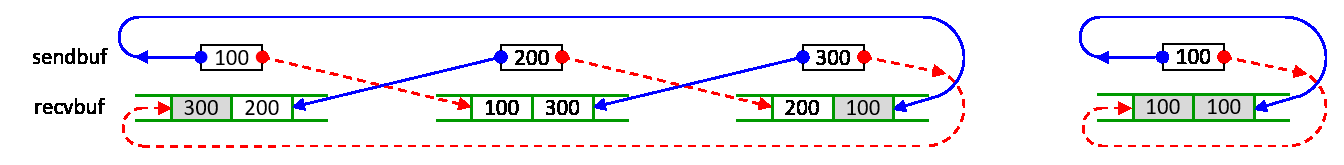
\includegraphics[width=6.0in]{figures/cart_neighbor_allgather}}
  \caption{Cartesian neighborhood allgather example for 3 and 1 processes in a dimension}
  \label{fig:cart-neighbor-allgather}
\end{figure}

The vector variant of \mpifunc{MPI\_NEIGHBOR\_ALLGATHER} allows one to gather
different numbers of elements from each neighbor.

\begin{mpi-binding}
    function_name("MPI_Neighbor_allgatherv")
    
    parameter(
        "sendbuf",
        "BUFFER",
        constant=True,
        desc=r"starting address of send buffer",
    )
    parameter(
        "sendcount",
        "POLYXFER_NUM_ELEM_NNI",
        desc=r"number of elements sent to each neighbor",
    )
    parameter("sendtype", "DATATYPE", desc=r"datatype of send buffer elements")
    parameter(
        "recvbuf",
        "BUFFER",
        direction="out",
        desc=r"starting address of receive buffer",
    )
    parameter(
        "recvcounts",
        "POLYXFER_NUM_ELEM_NNI",
        length="*",
        constant=True,
        desc=r"nonnegative integer array (of length indegree) "
        "containing the number of elements that are received "
        "from each neighbor",
        suppress="lis_paren",
    )
    parameter(
        "displs",
        "POLYDISPLACEMENT",
        constant=True,
        length="*",
        desc=r"integer array (of length indegree). Entry \mpicode{i} "
        r"specifies the displacement (relative to \mpiarg{recvbuf}) "
        r"at which to place the incoming data from neighbor "
        r"\mpicode{i}",
        suppress="lis_paren",
    )
    parameter(
        "recvtype", "DATATYPE", desc=r"datatype of receive buffer elements"
    )
    parameter(
        "comm", "COMMUNICATOR", desc=r"communicator with associated virtual topology"
    )
\end{mpi-binding}

The \mpifuncskip{MPI\_NEIGHBOR\_ALLGATHERV} procedure supports Cartesian communicators, graph communicators, and
distributed graph communicators as described
in \sectionref{sec:sparsecoll}.
If \mpiarg{comm} is a distributed graph communicator, the outcome is as if each
\MPI/ process executed sends to each of its outgoing neighbors and receives from
each of its incoming neighbors:

%%HEADER
%%LANG: C
%%FRAGMENT
%%DECL: int indegree, outdegree, weighted;
%%DECL: MPI_Comm comm; MPI_Request r; MPI_Datatype sendtype, recvtype;
%%DECL: int sendbuf[1], recvbuf[1], sendcount, recvcounts[1], displs[1];
%%DECL: int extent(MPI_Datatype);
%%SUBST:dsts\[k\],\.\.\.:dsts[k],0,comm,&r
%%SUBST:srcs\[k\],\.\.\.:srcs[k],0,comm,&r
%%SUBST:all\(\.\.\.:all(1,&r,MPI_STATUSES_IGNORE
%%ENDHEADER
\begin{lstlisting}[language={[MPI]C}]
MPI_Dist_graph_neighbors_count(comm, &indegree, &outdegree, &weighted);
int *srcs=(int*)malloc(indegree*sizeof(int));
int *dsts=(int*)malloc(outdegree*sizeof(int));
MPI_Dist_graph_neighbors(comm, indegree, srcs, MPI_UNWEIGHTED,
                         outdegree, dsts, MPI_UNWEIGHTED);
int k;

/* assume sendbuf and recvbuf are of type (char*) */
for(k=0; k<outdegree; ++k) 
  MPI_Isend(sendbuf, sendcount, sendtype, dsts[k],...); 

for(k=0; k<indegree; ++k) 
  MPI_Irecv(recvbuf+displs[k]*extent(recvtype), recvcounts[k], recvtype,
            srcs[k],...); 

MPI_Waitall(...);
\end{lstlisting}

The type signature associated with \mpiarg{sendcount}, \mpiarg{sendtype} at
\MPI/ process $j$ must be equal to the type signature associated with
\mpiarg{recvcounts}\mpicode{[l]}, \mpiarg{recvtype} at any other \MPI/ process
with \mpicode{srcs[l]=$j$}.
This implies that the amount of data sent must be equal to the
amount of data received, pairwise between every pair of
communicating \MPI/ processes.
Distinct type maps between sender and receiver are still allowed.
The data received from the \mpicode{l}-th neighbor is placed into
\mpiarg{recvbuf} beginning at offset \mpiarg{displs}\mpicode{[l]}
elements (in terms of the \mpiarg{recvtype}). 

The ``in place'' option is not meaningful for this operation.

All arguments are significant on all \MPI/ processes and the argument
\mpishortarg{comm} must have identical values on all \MPI/ processes.


\subsection{Neighborhood Alltoall}
\label{subsec:sparsecoll:alltoall}

In the neighborhood alltoall operation, each \MPI/ process $i$ receives data items from each \MPI/ process
$j$ if an edge $(j,i)$ exists in the topology graph or Cartesian
topology. Similarly, each \MPI/ process $i$ sends data items to all \MPI/ processes
$j$ where an edge $(i,j)$ exists. This call is more general than
\mpifunc{MPI\_NEIGHBOR\_ALLGATHER} in that different data items can be
sent to each neighbor. The $k$-th block in send buffer is sent to the
$k$-th neighboring \MPI/ process and the $l$-th block in the receive buffer is
received from the $l$-th neighbor.

\begin{mpi-binding}
    function_name("MPI_Neighbor_alltoall")
    
    parameter(
        "sendbuf",
        "BUFFER",
        constant=True,
        desc=r"starting address of send buffer",
    )
    parameter(
        "sendcount",
        "POLYXFER_NUM_ELEM_NNI",
        desc=r"number of elements sent to each neighbor",
    )
    parameter("sendtype", "DATATYPE", desc=r"datatype of send buffer elements")
    parameter(
        "recvbuf",
        "BUFFER",
        direction="out",
        desc=r"starting address of receive buffer",
    )
    parameter(
        "recvcount",
        "POLYXFER_NUM_ELEM_NNI",
        desc=r"number of elements received from each neighbor",
    )
    parameter(
        "recvtype", "DATATYPE", desc=r"datatype of receive buffer elements"
    )
    parameter(
        "comm", "COMMUNICATOR", desc=r"communicator with associated virtual topology"
    )
\end{mpi-binding}

The \mpifuncskip{MPI\_NEIGHBOR\_ALLTOALL} procedure supports Cartesian communicators, graph communicators, and
distributed graph communicators as described
in \sectionref{sec:sparsecoll}.
If \mpiarg{comm} is a distributed graph communicator, the outcome is as if each
\MPI/ process executed sends to each of its outgoing neighbors and receives from
each of its incoming neighbors:

%%HEADER
%%LANG: C
%%FRAGMENT
%%DECL: MPI_Comm comm; int indegree, outdegree, weighted;
%%DECL: MPI_Request r;
%%DECL: int sendbuf[1], sendcount, recvbuf[1], recvcount;
%%DECL: MPI_Datatype recvtype, sendtype;
%%DECL: int extent(MPI_Datatype);
%%SUBST:dsts\[k\],\.\.\.:dsts[k],0,comm,&r
%%SUBST:srcs\[k\],\.\.\.:srcs[k],0,comm,&r
%%SUBST:\(\.\.\.:(1,&r,MPI_STATUSES_IGNORE
%%ENDHEADER
\begin{lstlisting}[language={[MPI]C}]
MPI_Dist_graph_neighbors_count(comm, &indegree, &outdegree, &weighted);
int *srcs=(int*)malloc(indegree*sizeof(int));
int *dsts=(int*)malloc(outdegree*sizeof(int));
MPI_Dist_graph_neighbors(comm, indegree, srcs, MPI_UNWEIGHTED,
                         outdegree, dsts, MPI_UNWEIGHTED);
int k;

/* assume sendbuf and recvbuf are of type (char*) */
for(k=0; k<outdegree; ++k)
  MPI_Isend(sendbuf+k*sendcount*extent(sendtype), sendcount, sendtype,
            dsts[k],...); 

for(k=0; k<indegree; ++k)
  MPI_Irecv(recvbuf+k*recvcount*extent(recvtype), recvcount, recvtype,
            srcs[k],...);

MPI_Waitall(...);
\end{lstlisting}

The type signature associated with \mpiarg{sendcount}, \mpiarg{sendtype}
at an \MPI/ process must be equal to the type signature associated with
\mpiarg{recvcount}, \mpiarg{recvtype} at any other \MPI/ process.
This implies that the amount of data sent must be equal to the
amount of data received, pairwise between every pair of
communicating \MPI/ processes.
Distinct type maps between sender and receiver are still allowed.
 
The ``in place'' option is not meaningful for this operation.

All arguments are significant on all \MPI/ processes and the argument
\mpishortarg{comm} must have identical values on all \MPI/ processes.

\begin{example}
\label{cart-alltoall-exa}
\exindex{MPI\_Neighbor\_alltoall}%
\Exindex{Neutral}{Neighbor alltoall}{MPI\_NEIGHBOR\_ALLTOALL,MPI\_CARTDIM\_GET,MPI\_CART\_SHIFT,MPI\_SENDRECV}%
Buffer usage of \mpifunc{MPI\_NEIGHBOR\_ALLTOALL} in the case of a Cartesian virtual topology.

For a halo communication on a Cartesian grid, the buffer usage
in a given direction \mpicode{d} with  \mpicode{dims[d]=3} and  \mpicode{1}, 
respectively during creation of the communicator is described
in Figure~\ref{fig:cart-neighbor-alltoall}.

The figure may apply to any (or multiple) directions in
the Cartesian topology. The grey buffers are required in all
cases but are only accessed if during creation of the communicator,
\mpicode{periods[d]} was defined as nonzero (in C) or \mpicode{.TRUE.} (in Fortran).

If \mpiarg{sendbuf} and \mpiarg{recvbuf} are declared as \mpicode(char *) and contain a sequence of buffers
each described by \mpiarg{sendcount},\mpiarg{sendtype} and
\mpiarg{recvbuf},\mpiarg{recvtype}, then after \mpifunc{MPI\_NEIGHBOR\_ALLTOALL} on a Cartesian communicator returned, the content
of the \mpiarg{recvbuf} is as if the following code is executed:

%%HEADER
%%LANG: C
%% FIXME: mpichk needs to be updated to understand escapeinside
%%FRAGMENT
%%DECL: MPI_Comm comm; int ndims, d, rank_source, rank_dest;
%%DECL: MPI_Aint send_lb, send_extent, recv_lb, recv_extent;
%%DECL: char *sendbuf, *recvbuf;
%%DECL: int sendcount, recvcount;
%%DECL: MPI_Datatype recvtype, sendtype;
%%DECL: MPI_Status status;
%%ENDHEADER
\begin{lstlisting}[language={[MPI]C},basicstyle=\lstsmall,escapeinside=`']
MPI_Cartdim_get(comm, &ndims);
MPI_Type_get_extent(sendtype, &send_lb, &send_extent);
MPI_Type_get_extent(recvtype, &recv_lb, &recv_extent);
for( /*direction*/ d=0; d < ndims; d++) {
    MPI_Cart_shift(comm, /*direction*/ d, /*disp*/ 1, &rank_source, &rank_dest);
    MPI_Sendrecv(sendbuf+(d*2`\underline{+0}')*sendcount*send_extent,
                                 sendcount,sendtype,`\underline{rank\_source}',/*sendtag*/d*2,
                 recvbuf+(d*2`\underline{+1}')*recvcount*recv_extent,
                                 recvcount,recvtype,`\underline{rank\_dest}', /*recvtag*/ d*2,
                 comm,&status);/*communication in direction of displacment -1*/
    MPI_Sendrecv(sendbuf+(d*2`\underline{+1}')*sendcount*send_extent,
                                 sendcount,sendtype,`\underline{rank\_dest}', /*sendtag*/ d*2+1,
                 recvbuf+(d*2`\underline{+0}')*recvcount*recv_extent,
                                 recvcount,recvtype,`\underline{rank\_source}',/*recvtag*/d*2+1,
                 comm,&status);/*communication in direction of displacment +1*/
}
\end{lstlisting}

The first call to \mpicode{MPI\_Sendrecv} implements the solid arrows' communication pattern
in each diagram of Figure~\ref{fig:cart-neighbor-alltoall}, whereas the second call is for
the dashed arrows' pattern.
\end{example}

\begin{figure}
  \centerline{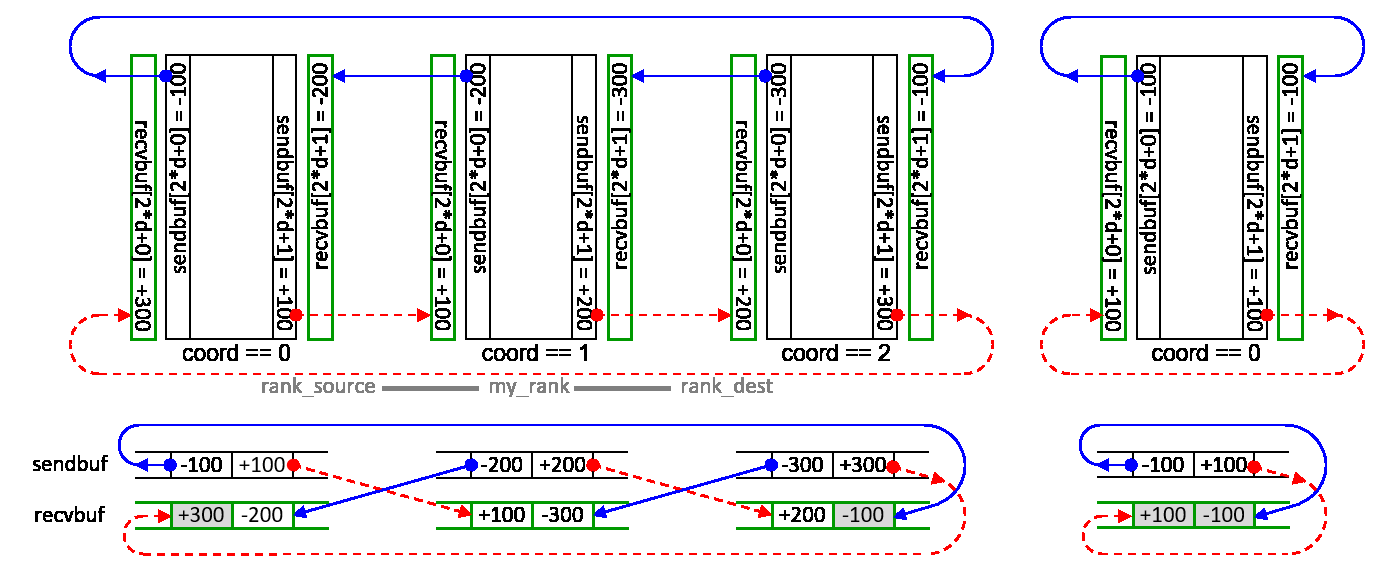
\includegraphics[width=6.0in]{figures/cart_neighbor_alltoall}}
  \caption{Cartesian neighborhood alltoall example for 3 and 1 \MPI/ processes in a dimension}
  \label{fig:cart-neighbor-alltoall}
\end{figure}

\begin{implementors}
For a Cartesian topology, if the grid in a
direction \mpicode{d} is periodic and \mpicode{dims[d]} is equal to 1 or 2,
then \mpicode{rank\_source} and \mpicode{rank\_dest} are identical, 
but still all \mpicode{ndims} send and \mpicode{ndims} receive operations
use different buffers. 
If in this case, the two send and receive operations per direction or
of all directions are internally parallelized, then the several send and
receive operations for the same sender-receiver \MPI/ process pair shall be
initiated in the same sequence on sender and receiver side or
they shall be distinguished by different tags.
The code above shows a valid sequence of operations and tags.
\end{implementors}

The vector variant of \mpifunc{MPI\_NEIGHBOR\_ALLTOALL} allows
sending/receiving different numbers of elements to and from each neighbor.

\begin{mpi-binding}
    function_name("MPI_Neighbor_alltoallv")
    
    parameter(
        "sendbuf",
        "BUFFER",
        constant=True,
        desc=r"starting address of send buffer",
    )
    parameter(
        "sendcounts",
        "POLYXFER_NUM_ELEM_NNI",
        constant=True,
        length="*",
        desc=r"nonnegative integer array (of length outdegree) "
        "specifying the number of elements to send to each "
        "neighbor",
        suppress="lis_paren",
    )
    parameter(
        "sdispls",
        "POLYDISPLACEMENT",
        constant=True,
        length="*",
        desc=r"integer array (of length outdegree). Entry "
        r"\mpicode{j} specifies the displacement (relative to "
        r"\mpiarg{sendbuf}) from which to send the outgoing "
        r"data to neighbor \mpicode{j}",
        suppress="lis_paren",
    )
    parameter("sendtype", "DATATYPE", desc=r"datatype of send buffer elements")
    parameter(
        "recvbuf",
        "BUFFER",
        direction="out",
        desc=r"starting address of receive buffer",
    )
    parameter(
        "recvcounts",
        "POLYXFER_NUM_ELEM_NNI",
        constant=True,
        length="*",
        desc=r"nonnegative integer array (of length indegree) "
        "specifying the number of elements that are received "
        "from each neighbor",
        suppress="lis_paren",
    )
    parameter(
        "rdispls",
        "POLYDISPLACEMENT",
        constant=True,
        length="*",
        desc=(
            r"integer array (of length indegree). Entry "
            r"\mpicode{i} specifies the displacement (relative "
            r"to \mpiarg{recvbuf}) at which to place the incoming "
            r"data from neighbor \mpicode{i}"
        ),
        suppress="lis_paren",
    )
    parameter(
        "recvtype", "DATATYPE", desc=r"datatype of receive buffer elements"
    )
    parameter(
        "comm", "COMMUNICATOR", desc=r"communicator with associated virtual topology"
    )
\end{mpi-binding}

\begin{sloppy}
The \mpifuncskip{MPI\_NEIGHBOR\_ALLTOALLV} procedure supports Cartesian communicators, graph communicators, and
distributed graph communicators as described
in \sectionref{sec:sparsecoll}.
If \mpiarg{comm} is a distributed graph communicator, the outcome is as if each
\MPI/ process executed sends to each of its outgoing neighbors and receives from
each of its incoming neighbors:

\end{sloppy}
%%HEADER
%%LANG: C
%%FRAGMENT
%%DECL: MPI_Comm comm; int indegree, outdegree, weighted; 
%%DECL: int sendbuf[1], sdispls[1], sendcounts[1], recvbuf[1], rdispls[1];
%%DECL: int recvcounts[1];  MPI_Datatype sendtype, recvtype; MPI_Request r;
%%DECL: int extent(MPI_Datatype);
%%SUBST:dsts\[k\],\.\.\.:dsts[k],0,comm,&r
%%SUBST:srcs\[k\],\.\.\.:srcs[k],0,comm,&r
%%SUBST:\(\.\.\.\):(1,&r,MPI_STATUSES_IGNORE)
%%ENDHEADER
\begin{lstlisting}[language={[MPI]C}]
MPI_Dist_graph_neighbors_count(comm, &indegree, &outdegree, &weighted);
int *srcs=(int*)malloc(indegree*sizeof(int));
int *dsts=(int*)malloc(outdegree*sizeof(int));
MPI_Dist_graph_neighbors(comm, indegree, srcs, MPI_UNWEIGHTED,
                         outdegree, dsts, MPI_UNWEIGHTED);
int k;

/* assume sendbuf and recvbuf are of type (char*) */
for(k=0; k<outdegree; ++k)
  MPI_Isend(sendbuf+sdispls[k]*extent(sendtype), sendcounts[k],
            sendtype, dsts[k],...);

for(k=0; k<indegree; ++k)
  MPI_Irecv(recvbuf+rdispls[k]*extent(recvtype), recvcounts[k],
            recvtype, srcs[k],...);

MPI_Waitall(...);
\end{lstlisting}

The type signature associated with
\mpiarg{sendcounts}\mpicode{[k]}, \mpiarg{sendtype}
with \mpicode{dsts[k]=$j$} at \MPI/ process $i$
must be equal to the type signature associated with
\mpiarg{recvcounts}\mpicode{[l]}, \mpiarg{recvtype}
with \mpicode{srcs[l]=$i$} at \MPI/ process $j$.
This implies that the amount of data sent must be equal to the
amount of data received, pairwise between every pair of
communicating \MPI/ processes.
Distinct type maps between sender and receiver are still allowed.
The data in the \mpiarg{sendbuf} beginning at offset 
\mpiarg{sdispls}\mpicode{[k]} elements (in terms of the \mpiarg{sendtype}) 
is sent to the \mpicode{k}-th outgoing neighbor.
The data received from the \mpicode{l}-th incoming neighbor is placed
into \mpiarg{recvbuf} beginning at offset \mpiarg{rdispls}\mpicode{[l]}
elements (in terms of the \mpiarg{recvtype}). 
 
The ``in place'' option is not meaningful for this operation.

All arguments are significant on all \MPI/ processes and the argument
\mpishortarg{comm} must have identical values on all \MPI/ processes.


\mpifunc{MPI\_NEIGHBOR\_ALLTOALLW} allows one to send and receive with
different datatypes to and from each neighbor.

\begin{mpi-binding}
    function_name("MPI_Neighbor_alltoallw")
    parameter(
        "sendbuf",
        "BUFFER",
        desc=r"starting address of send buffer",
        constant=True,
    )
    parameter(
        "sendcounts",
        "POLYXFER_NUM_ELEM_NNI",
        desc=(
            r"nonnegative integer array (of length outdegree) specifying "
            r"the number of elements to send to each neighbor"
        ),
        constant=True,
        length="*",
        suppress="lis_paren",
    )
    parameter(
        "sdispls",
        "DISPLACEMENT",
        desc=(
            r"integer array (of length outdegree). Entry \mpicode{j} "
            r"specifies the displacement in bytes (relative to "
            r"\mpiarg{sendbuf}) from which to take the outgoing data "
            r"destined for neighbor \mpicode{j}"
        ),
        constant=True,
        length="*",
    )
    parameter(
        "sendtypes",
        "DATATYPE",
        desc=(
            r"array of datatypes (of length outdegree). Entry \mpicode{j} "
            r"specifies the type of data to send to neighbor \mpicode{j}"
        ),
        constant=True,
        length="*",
    )
    parameter(
        "recvbuf",
        "BUFFER",
        desc=r"starting address of receive buffer",
        direction="out",
    )
    parameter(
        "recvcounts",
        "POLYXFER_NUM_ELEM_NNI",
        desc=(
            r"nonnegative integer array (of length indegree) specifying the "
            r"number of elements that are received from each neighbor"
        ),
        constant=True,
        length="*",
        suppress="lis_paren",
    )
    parameter(
        "rdispls",
        "DISPLACEMENT",
        desc=(
            r"integer array (of length indegree). Entry \mpicode{i} "
            r"specifies the displacement in bytes (relative to "
            r"\mpiarg{recvbuf}) at which to place the incoming data "
            r"from neighbor \mpicode{i}"
        ),
        constant=True,
        length="*",
    )
    parameter(
        "recvtypes",
        "DATATYPE",
        desc=(
            r"array of datatypes (of length indegree). Entry \mpicode{i} "
            r"specifies the type of data received from neighbor \mpicode{i}"
        ),
        constant=True,
        length="*",
    )
    parameter(
        "comm", "COMMUNICATOR", desc=r"communicator with associated virtual topology"
    )
\end{mpi-binding}

The \mpifuncskip{MPI\_NEIGHBOR\_ALLTOALLW} procedure supports Cartesian communicators, \gb{}graph communicators, and
distributed graph communicators as described
in \sectionref{sec:sparsecoll}.
If \mpiarg{comm} is a distributed graph communicator, the outcome is as if each
\MPI/ process executed sends to each of its outgoing neighbors and receives from
each of its incoming neighbors:

%%HEADER
%%LANG: C
%%FRAGMENT
%%DECL: MPI_Comm comm; int indegree, outdegree, weighted; MPI_Request r;
%%DECL: int sendbuf[1], sdispls[1], sendcounts[1], recvbuf[1], rdispls[1];
%%DECL: int recvcounts[1];  MPI_Datatype sendtypes[1], recvtypes[1];
%%SUBST:dsts\[k\],\.\.\.:dsts[k],0,comm,&r
%%SUBST:srcs\[k\],\.\.\.:srcs[k],0,comm,&r
%%SUBST:\(\.\.\.\):(1,&r,MPI_STATUSES_IGNORE)
%%ENDHEADER
\begin{lstlisting}[language={[MPI]C}]
MPI_Dist_graph_neighbors_count(comm, &indegree, &outdegree, &weighted);
int *srcs=(int*)malloc(indegree*sizeof(int));
int *dsts=(int*)malloc(outdegree*sizeof(int));
MPI_Dist_graph_neighbors(comm, indegree, srcs, MPI_UNWEIGHTED,
                         outdegree, dsts, MPI_UNWEIGHTED);
int k;

/* assume sendbuf and recvbuf are of type (char*) */
for(k=0; k<outdegree; ++k)
  MPI_Isend(sendbuf+sdispls[k], sendcounts[k], sendtypes[k],
            dsts[k],...);

for(k=0; k<indegree; ++k)
  MPI_Irecv(recvbuf+rdispls[k], recvcounts[k], recvtypes[k],
            srcs[k],...);

MPI_Waitall(...);
\end{lstlisting}

The type signature associated with
\mpiarg{sendcounts}\mpicode{[k]}, \mpiarg{sendtypes}\mpicode{[k]}
with \mpicode{dsts[k]=$j$} at \MPI/ process $i$
must be equal to the type signature associated with
\mpiarg{recvcounts}\mpicode{[l]}, \mpiarg{recvtypes}\mpicode{[l]}
with \mpicode{srcs[l]=$i$} at \MPI/ process $j$.
This implies that the amount of data sent must be equal to the
amount of data received, pairwise between every pair of
communicating \MPI/ processes.
Distinct type maps between sender and receiver are still allowed.
 
The ``in place'' option is not meaningful for this operation.

All arguments are significant on all \MPI/ processes and the argument
\mpishortarg{comm} must have identical values on all \MPI/ processes.



%% The full running head is too long for the page
\section[Nonblocking Neighborhood Communication]{Nonblocking Neighborhood Communication on Process Topologies}
\label{sec:sparsecoll-nbc}

Nonblocking variants of the neighborhood collective operations allow
relaxed synchronization and
overlapping of computation and communication.
The semantics are similar to nonblocking collective
operations as described in Section~\ref{sec:nbcoll}. 

\subsection{Nonblocking Neighborhood Gather}
\mpitermtitleindex{neighborhood collective communication!nonblocking}

\begin{mpi-binding}
    function_name("MPI_Ineighbor_allgather")
    parameter(
        "sendbuf",
        "BUFFER",
        desc=r"starting address of send buffer",
        constant=True,
        asynchronous=True,
    )
    parameter(
        "sendcount",
        "POLYXFER_NUM_ELEM_NNI",
        desc=r"number of elements sent to each neighbor",
    )
    parameter("sendtype", "DATATYPE", desc=r"datatype of send buffer elements")
    parameter(
        "recvbuf",
        "BUFFER",
        desc=r"starting address of receive buffer",
        direction="out",
        suppress="f08_intent",
        asynchronous=True,
    )
    parameter(
        "recvcount",
        "POLYXFER_NUM_ELEM_NNI",
        desc=r"number of elements received from each neighbor",
    )
    parameter(
        "recvtype", "DATATYPE", desc=r"datatype of receive buffer elements"
    )
    parameter(
        "comm", "COMMUNICATOR", desc=r"communicator with associated virtual topology"
    )
    parameter(
        "request", "REQUEST", desc=r"communication request", direction="out"
    )
\end{mpi-binding}

\mpifuncskip{MPI\_INEIGHBOR\_ALLGATHER} starts a nonblocking variant of
\mpifunc{MPI\_NEIGHBOR\_ALLGATHER}.

\begin{mpi-binding}
    function_name("MPI_Ineighbor_allgatherv")
    parameter(
        "sendbuf",
        "BUFFER",
        desc=r"starting address of send buffer",
        constant=True,
        asynchronous=True,
    )
    parameter(
        "sendcount",
        "POLYXFER_NUM_ELEM_NNI",
        desc=r"number of elements sent to each neighbor",
    )
    parameter("sendtype", "DATATYPE", desc=r"datatype of send buffer elements")
    parameter(
        "recvbuf",
        "BUFFER",
        desc=r"starting address of receive buffer",
        direction="out",
        suppress="f08_intent",
        asynchronous=True,
    )
    parameter(
        "recvcounts",
        "POLYXFER_NUM_ELEM_NNI",
        desc=(
            r"nonnegative integer array (of length indegree) containing the "
            r"number of elements that are received from each neighbor"
        ),
        constant=True,
        asynchronous=True,
        length="*",
        suppress="lis_paren",
    )
    parameter(
        "displs",
        "POLYDISPLACEMENT",
        desc=(
            r"integer array (of length indegree). Entry \mpicode{i} "
            r"specifies the displacement (relative to \mpiarg{recvbuf}) at "
            r"rwhich to place the incoming data from neighbor \mpicode{i}"
        ),
        constant=True,
        length="*",
        asynchronous=True,
        suppress="lis_paren",
    )
    parameter(
        "recvtype", "DATATYPE", desc=r"datatype of receive buffer elements"
    )
    parameter(
        "comm", "COMMUNICATOR", desc=r"communicator with associated virtual topology"
    )
    parameter(
        "request", "REQUEST", desc=r"communication request", direction="out"
    )
\end{mpi-binding}

%
\mpifuncskip{MPI\_INEIGHBOR\_ALLGATHERV} starts a nonblocking variant of
\mpifunc{MPI\_NEIGHBOR\_ALLGATHERV}.

\subsection{Nonblocking Neighborhood Alltoall}

\begin{mpi-binding}
    function_name("MPI_Ineighbor_alltoall")
    parameter(
        "sendbuf",
        "BUFFER",
        desc=r"starting address of send buffer",
        constant=True,
        asynchronous=True,
    )
    parameter(
        "sendcount",
        "POLYXFER_NUM_ELEM_NNI",
        desc=r"number of elements sent to each neighbor",
    )
    parameter("sendtype", "DATATYPE", desc=r"datatype of send buffer elements")
    parameter(
        "recvbuf",
        "BUFFER",
        desc=r"starting address of receive buffer",
        direction="out",
        suppress="f08_intent",
        asynchronous=True,
    )
    parameter(
        "recvcount",
        "POLYXFER_NUM_ELEM_NNI",
        desc=r"number of elements received from each neighbor",
    )
    parameter(
        "recvtype", "DATATYPE", desc=r"datatype of receive buffer elements"
    )
    parameter(
        "comm", "COMMUNICATOR", desc=r"communicator with associated virtual topology"
    )
    parameter(
        "request", "REQUEST", desc=r"communication request", direction="out"
    )
\end{mpi-binding}

\mpifuncskip{MPI\_INEIGHBOR\_ALLTOALL} starts a nonblocking variant of
\mpifunc{MPI\_NEIGHBOR\_ALLTOALL}.


\begin{mpi-binding}
    function_name("MPI_Ineighbor_alltoallv")
    parameter(
        "sendbuf",
        "BUFFER",
        desc=r"starting address of send buffer",
        constant=True,
        asynchronous=True,
    )
    parameter(
        "sendcounts",
        "POLYXFER_NUM_ELEM_NNI",
        desc=(
            r"nonnegative integer array (of length outdegree) specifying "
            r"the number of elements to send to each neighbor"
        ),
        constant=True,
        asynchronous=True,
        length="*",
        suppress="lis_paren",
    )
    parameter(
        "sdispls",
        "POLYDISPLACEMENT",
        desc=(
            r"integer array (of length outdegree). Entry \mpicode{j} "
            r"specifies the displacement (relative to \mpiarg{sendbuf}) "
            r"from which send the outgoing data to neighbor \mpicode{j}"
        ),
        constant=True,
        length="*",
        asynchronous=True,
        suppress="lis_paren",
    )
    parameter("sendtype", "DATATYPE", desc=r"datatype of send buffer elements")
    parameter(
        "recvbuf",
        "BUFFER",
        desc=r"starting address of receive buffer",
        direction="out",
        suppress="f08_intent",
        asynchronous=True,
    )
    parameter(
        "recvcounts",
        "POLYXFER_NUM_ELEM_NNI",
        desc=(
            r"nonnegative integer array (of length indegree) specifying the "
            r"number of elements that are received from each neighbor"
        ),
        constant=True,
        length="*",
        asynchronous=True,
        suppress="lis_paren",
    )
    parameter(
        "rdispls",
        "POLYDISPLACEMENT",
        desc=(
            r"integer array (of length indegree). Entry \mpicode{i} "
            r"specifies the displacement (relative to \mpiarg{recvbuf}) at "
            r"which to place the incoming data from neighbor \mpicode{i}"
        ),
        constant=True,
        length="*",
        asynchronous=True,
        suppress="lis_paren",
    )
    parameter(
        "recvtype", "DATATYPE", desc=r"datatype of receive buffer elements"
    )
    parameter(
        "comm", "COMMUNICATOR", desc=r"communicator with associated virtual topology"
    )
    parameter(
        "request", "REQUEST", desc=r"communication request", direction="out"
    )
\end{mpi-binding}

\mpifuncskip{MPI\_INEIGHBOR\_ALLTOALLV} starts a nonblocking variant of
\mpifunc{MPI\_NEIGHBOR\_ALLTOALLV}.

\begin{mpi-binding}
    function_name("MPI_Ineighbor_alltoallw")
    parameter(
        "sendbuf",
        "BUFFER",
        desc=r"starting address of send buffer",
        constant=True,
        asynchronous=True,
    )
    parameter(
        "sendcounts",
        "POLYXFER_NUM_ELEM_NNI",
        desc=(
            r"nonnegative integer array (of length outdegree) specifying "
            r"the number of elements to send to each neighbor"
        ),
        constant=True,
        asynchronous=True,
        length="*",
        suppress="lis_paren",
    )
    parameter(
        "sdispls",
        "DISPLACEMENT",
        desc=(
            r"integer array (of length outdegree). Entry \mpicode{j} "
            r"specifies the displacement in bytes (relative to "
            r"\mpiarg{sendbuf}) from which to take the outgoing data "
            r"destined for neighbor \mpicode{j}"
        ),
        constant=True,
        asynchronous=True,
        length="*",
    )
    parameter(
        "sendtypes",
        "DATATYPE",
        desc=(
            r"array of datatypes (of length outdegree). Entry "
            r"\mpicode{j} specifies the type of data to send to neighbor "
            r"\mpicode{j}"
        ),
        constant=True,
        asynchronous=True,
        length="*",
    )
    parameter(
        "recvbuf",
        "BUFFER",
        desc=r"starting address of receive buffer",
        direction="out",
        suppress="f08_intent",
        asynchronous=True,
    )
    parameter(
        "recvcounts",
        "POLYXFER_NUM_ELEM_NNI",
        desc=(
            r"nonnegative integer array (of length indegree) specifying the "
            r"number of elements that are received from each neighbor"
        ),
        constant=True,
        length="*",
        asynchronous=True,
        suppress="lis_paren",
    )
    parameter(
        "rdispls",
        "DISPLACEMENT",
        desc=(
            r"integer array (of length indegree). Entry \mpicode{i} specifies "
            r"the displacement in bytes (relative to \mpiarg{recvbuf}) at "
            r"which to place the incoming data from neighbor \mpicode{i}"
        ),
        constant=True,
        length="*",
        asynchronous=True,
    )
    parameter(
        "recvtypes",
        "DATATYPE",
        desc=(
            r"array of datatypes (of length indegree). Entry \mpicode{i} "
            r"specifies the type of data received from neighbor \mpicode{i}"
        ),
        constant=True,
        length="*",
        asynchronous=True,
    )
    parameter(
        "comm", "COMMUNICATOR", desc=r"communicator with associated virtual topology"
    )
    parameter(
        "request", "REQUEST", desc=r"communication request", direction="out"
    )
\end{mpi-binding}

\mpifuncskip{MPI\_INEIGHBOR\_ALLTOALLW} starts a nonblocking variant of
\mpifunc{MPI\_NEIGHBOR\_ALLTOALLW}.

% include persistent neighbor collectives
%% The full running head is too long for the page
\section[Persistent Neighborhood Communication]{Persistent Neighborhood Communication on Process Topologies}
\mpitermtitleindex{persistent communication requests!collective persistent}
\label{sec:sparsecoll-pnbc}

Persistent variants of the neighborhood collective operations can offer
significant performance benefits for programs with repetitive communication
patterns. The semantics are similar to persistent collective
operations as described in Section~\ref{sec:coll-persistent}. 

\subsection{Persistent Neighborhood Gather}

\begin{mpi-binding}
    function_name("MPI_Neighbor_allgather_init")
    parameter(
        "sendbuf",
        "BUFFER",
        desc=r"starting address of send buffer",
        constant=True,
        asynchronous=True,
    )
    parameter(
        "sendcount",
        "POLYXFER_NUM_ELEM_NNI",
        desc=r"number of elements sent to each neighbor",
    )
    parameter("sendtype", "DATATYPE", desc=r"datatype of send buffer elements")
    parameter(
        "recvbuf",
        "BUFFER",
        desc=r"starting address of receive buffer",
        direction="out",
        suppress="f08_intent",
        asynchronous=True,
    )
    parameter(
        "recvcount",
        "POLYXFER_NUM_ELEM_NNI",
        desc=r"number of elements received from each neighbor",
    )
    parameter(
        "recvtype", "DATATYPE", desc=r"datatype of receive buffer elements"
    )
    parameter(
        "comm", "COMMUNICATOR", desc=r"communicator with associated virtual topology"
    )
    parameter("info", "INFO", desc=r"info argument")
    parameter(
        "request", "REQUEST", desc=r"communication request", direction="out"
    )
\end{mpi-binding}

Creates a persistent collective communication request for the neighborhood allgather operation. 

\begin{mpi-binding}
    function_name("MPI_Neighbor_allgatherv_init")
    parameter(
        "sendbuf",
        "BUFFER",
        desc=r"starting address of send buffer",
        constant=True,
        asynchronous=True,
    )
    parameter(
        "sendcount",
        "POLYXFER_NUM_ELEM_NNI",
        desc=r"number of elements sent to each neighbor",
    )
    parameter("sendtype", "DATATYPE", desc=r"datatype of send buffer elements")
    parameter(
        "recvbuf",
        "BUFFER",
        desc=r"starting address of receive buffer",
        direction="out",
        suppress="f08_intent",
        asynchronous=True,
    )
    parameter(
        "recvcounts",
        "POLYXFER_NUM_ELEM_NNI",
        desc=(
            r"nonnegative integer array (of length indegree) containing the "
            r"number of elements that are received from each neighbor"
        ),
        constant=True,
        asynchronous=True,
        length="*",
        suppress="lis_paren",
    )
    parameter(
        "displs",
        "POLYDISPLACEMENT",
        desc=(
            r"integer array (of length indegree). Entry \mpicode{i} "
            r"specifies the displacement (relative to \mpiarg{recvbuf}) "
            r"at which to place the incoming data from neighbor "
            r"\mpicode{i}"
        ),
        constant=True,
        length="*",
        suppress="lis_paren",
    )
    parameter(
        "recvtype", "DATATYPE", desc=r"datatype of receive buffer elements"
    )
    parameter(
        "comm", "COMMUNICATOR", desc=r"communicator with associated virtual topology"
    )
    parameter("info", "INFO", desc=r"info argument")
    parameter(
        "request", "REQUEST", desc=r"communication request", direction="out"
    )
\end{mpi-binding}

%
Creates a persistent collective communication request for the neighborhood allgatherv operation. 


\subsection{Persistent Neighborhood Alltoall}

\begin{mpi-binding}
    function_name("MPI_Neighbor_alltoall_init")
    parameter(
        "sendbuf",
        "BUFFER",
        desc=r"starting address of send buffer",
        constant=True,
        asynchronous=True,
    )
    parameter(
        "sendcount",
        "POLYXFER_NUM_ELEM_NNI",
        desc=r"number of elements sent to each neighbor",
    )
    parameter("sendtype", "DATATYPE", desc=r"datatype of send buffer elements")
    parameter(
        "recvbuf",
        "BUFFER",
        desc=r"starting address of receive buffer",
        direction="out",
        suppress="f08_intent",
        asynchronous=True,
    )
    parameter(
        "recvcount",
        "POLYXFER_NUM_ELEM_NNI",
        desc=r"number of elements received from each neighbor",
    )
    parameter(
        "recvtype", "DATATYPE", desc=r"datatype of receive buffer elements"
    )
    parameter(
        "comm", "COMMUNICATOR", desc=r"communicator with associated virtual topology"
    )
    parameter("info", "INFO", desc=r"info argument")
    parameter(
        "request", "REQUEST", desc=r"communication request", direction="out"
    )
\end{mpi-binding}

Creates a persistent collective communication request for the neighborhood alltoall operation. 

\begin{mpi-binding}
    function_name("MPI_Neighbor_alltoallv_init")
    parameter(
        "sendbuf",
        "BUFFER",
        desc=r"starting address of send buffer",
        constant=True,
        asynchronous=True,
    )
    parameter(
        "sendcounts",
        "POLYXFER_NUM_ELEM_NNI",
        desc=(
            r"nonnegative integer array (of length outdegree) specifying "
            r"the number of elements to send to each neighbor"
        ),
        constant=True,
        asynchronous=True,
        length="*",
        suppress="lis_paren",
    )
    parameter(
        "sdispls",
        "POLYDISPLACEMENT",
        desc=(
            r"integer array (of length outdegree). Entry \mpicode{j} "
            r"specifies the displacement (relative to \mpiarg{sendbuf}) "
            r"from which send the outgoing data to neighbor \mpicode{j}"
        ),
        constant=True,
        length="*",
        asynchronous=True,
        suppress="lis_paren",
    )
    parameter("sendtype", "DATATYPE", desc=r"datatype of send buffer elements")
    parameter(
        "recvbuf",
        "BUFFER",
        desc=r"starting address of receive buffer",
        direction="out",
        suppress="f08_intent",
        asynchronous=True,
    )
    parameter(
        "recvcounts",
        "POLYXFER_NUM_ELEM_NNI",
        desc=(
            r"nonnegative integer array (of length indegree) specifying the "
            r"number of elements that are received from each neighbor"
        ),
        constant=True,
        length="*",
        asynchronous=True,
        suppress="lis_paren",
    )
    parameter(
        "rdispls",
        "POLYDISPLACEMENT",
        desc=(
            r"integer array (of length indegree). Entry \mpicode{i} specifies "
            r"the displacement (relative to \mpiarg{recvbuf}) at which to "
            r"place the incoming data from neighbor \mpicode{i}"
        ),
        constant=True,
        length="*",
        asynchronous=True,
        suppress="lis_paren",
    )
    parameter(
        "recvtype", "DATATYPE", desc=r"datatype of receive buffer elements"
    )
    parameter(
        "comm", "COMMUNICATOR", desc=r"communicator with associated virtual topology"
    )
    parameter("info", "INFO", desc=r"info argument")
    parameter(
        "request", "REQUEST", desc=r"communication request", direction="out"
    )
\end{mpi-binding}

Creates a persistent collective communication request for the neighborhood alltoallv operation. 


\begin{mpi-binding}
    function_name("MPI_Neighbor_alltoallw_init")
    parameter(
        "sendbuf",
        "BUFFER",
        desc=r"starting address of send buffer",
        constant=True,
        asynchronous=True,
    )
    parameter(
        "sendcounts",
        "POLYXFER_NUM_ELEM_NNI",
        desc=(
            r"nonnegative integer array (of length outdegree) specifying "
            r"the number of elements to send to each neighbor"
        ),
        constant=True,
        asynchronous=True,
        length="*",
        suppress="lis_paren",
    )
    parameter(
        "sdispls",
        "DISPLACEMENT",
        desc=(
            r"integer array (of length outdegree). Entry \mpicode{j} "
            r"specifies the displacement in bytes (relative to "
            r"\mpiarg{sendbuf}) from which to take the outgoing data "
            r"destined for neighbor \mpicode{j}"
        ),
        constant=True,
        asynchronous=True,
        length="*",
    )
    parameter(
        "sendtypes",
        "DATATYPE",
        desc=(
            r"array of datatypes (of length outdegree). Entry \mpicode{j} "
            r"specifies the type of data to send to neighbor \mpicode{j}"
        ),
        constant=True,
        asynchronous=True,
        length="*",
    )
    parameter(
        "recvbuf",
        "BUFFER",
        desc=r"starting address of receive buffer",
        direction="out",
        suppress="f08_intent",
        asynchronous=True,
    )
    parameter(
        "recvcounts",
        "POLYXFER_NUM_ELEM_NNI",
        desc=(
            r"nonnegative integer array (of length indegree) specifying the "
            r"number of elements that are received from each neighbor"
        ),
        constant=True,
        length="*",
        asynchronous=True,
        suppress="lis_paren",
    )
    parameter(
        "rdispls",
        "DISPLACEMENT",
        desc=(
            r"integer array (of length indegree). Entry \mpicode{i} "
            r"specifies the displacement in bytes (relative to "
            r"\mpiarg{recvbuf}) at which to place the incoming data "
            r"from neighbor \mpicode{i}"
        ),
        constant=True,
        length="*",
        asynchronous=True,
    )
    parameter(
        "recvtypes",
        "DATATYPE",
        desc=(
            r"array of datatypes (of length indegree). Entry \mpicode{i} "
            r"specifies the type of data received from neighbor \mpicode{i}"
        ),
        constant=True,
        length="*",
        asynchronous=True,
    )
    parameter(
        "comm", "COMMUNICATOR", desc=r"communicator with associated virtual topology"
    )
    parameter("info", "INFO", desc=r"info argument")
    parameter(
        "request", "REQUEST", desc=r"communication request", direction="out"
    )
\end{mpi-binding}

Creates a persistent collective communication request for the neighborhood alltoallw operation. 

% TODO: Provide an example


\section{An Application Example}
\label{sec:topol-applic-example}

\begin{example}
\label{topol-exF}
\exindex{Topologies}%
\exindex{Virtual topologies}%
\exindex{Cartesian virtual topologies}%
\exindex{Neighborhood collective communication}%
\Exindex{Fortran}{Neighborhood collective communication}{MPI\_Dims\_create,MPI\_Cart\_create,MPI\_Cart\_get,MPI\_Cart\_shift,MPI\_Neighbor\_alltoall,MPI\_Neighbor\_alltoallw,MPI\_Neighbor\_alltoallw\_init}%
Neighborhood collective communication in a Cartesian virtual topology.

The example in 
Listings~\ref{poisson-begin}--\ref{poisson-persistent}
shows how the grid definition and
inquiry functions can be used in an application program. A partial
differential equation, for instance the Poisson equation, is to be
solved on a rectangular domain.
First, the \MPI/ processes organize themselves in a two-dimensional
structure. Each \MPI/ process then inquires about the ranks of its
neighbors in the four directions (up, down, right, left).
The numerical problem is solved by an iterative method, the details
of which are hidden in the subroutine \code{relax}.

In each relaxation step each \MPI/ process computes new values for the solution grid
function at the points \code{u(1:100,1:100)}
owned by the \MPI/ process. Then the values at inter-process
boundaries have to be exchanged with neighboring \MPI/ processes.
For example, the
newly calculated values in \code{u(1,1:100)}
must be sent into the halo cells \code{u(101,1:100)}
of the left-hand neighbor with coordinates \code{(own\_coord(1)-1,own\_coord(2))}.

%%HEADER
%%LANG: FORTRAN90
%%SKIPELIPSIS
%%FRAGMENT
%%DECL: interface
%%DECL: subroutine init(u,f)
%%DECL: real u(0:101,0:101), f(0:101,0:101)
%%DECL: end subroutine init
%%DECL: subroutine relax(u,f)
%%DECL: real u(0:101,0:101), f(0:101,0:101)
%%DECL: end subroutine relax
%%DECL: subroutine exchange(u,comm_cart,nrank,nneigh)
%%DECL: real u(0:101,0:101)
%%DECL: integer comm_cart, nrank(*), nneigh
%%DECL: end subroutine exchange
%%DECL: subroutine output(u)
%%DECL: real u(0:101,0:101)
%%DECL: end subroutine output
%%DECL: end interface
%%ENDHEADER
\begin{lstlisting}[language={[MPI]Fortran},basicstyle=\lstsmall,caption={Set-up of \MPI/ process structure for two-dimensional parallel Poisson solver},label=poisson-begin]
INTEGER ndims, num_neigh
LOGICAL reorder
PARAMETER (ndims=2, num_neigh=4, reorder=.true.)
INTEGER comm, comm_size, comm_cart, dims(ndims), ierr
INTEGER neigh_rank(num_neigh), own_coords(ndims), i, j, it
LOGICAL periods(ndims)
REAL u(0:101,0:101), f(0:101,0:101)
DATA dims / ndims * 0 /
comm = MPI_COMM_WORLD
CALL MPI_COMM_SIZE(comm, comm_size, ierr)
!   Set MPI process grid size and periodicity
CALL MPI_DIMS_CREATE(comm_size, ndims, dims, ierr)
periods(1) = .TRUE.
periods(2) = .TRUE.
!   Create a grid structure in WORLD group and inquire about own position
CALL MPI_CART_CREATE(comm, ndims, dims, periods, reorder, &
                     comm_cart, ierr)
CALL MPI_CART_GET(comm_cart, ndims, dims, periods, own_coords, ierr)
i = own_coords(1)
j = own_coords(2)
! Look up the ranks for the neighbors.  Own MPI process coordinates are (i,j).
! Neighbors are (i-1,j), (i+1,j), (i,j-1), (i,j+1) modulo (dims(1),dims(2))
CALL MPI_CART_SHIFT(comm_cart, 0,1, neigh_rank(1), neigh_rank(2), ierr)
CALL MPI_CART_SHIFT(comm_cart, 1,1, neigh_rank(3), neigh_rank(4), ierr)
! Initialize the grid functions and start the iteration
CALL init(u, f)
DO it=1,100
   CALL relax(u, f)
!      Exchange data with neighbor processes
   CALL exchange(u, comm_cart, neigh_rank, num_neigh)
END DO
CALL output(u)
\end{lstlisting}
%............................................................................


%............................................................................
%%HEADER
%%LANG: FORTRAN90
%%SUBST:\.\.\.:777, comm_cart, ierr
%%ENDHEADER
\begin{lstlisting}[language={[MPI]Fortran},basicstyle=\lstsmall,caption={Communication routine with local data copying and sparse neighborhood alltoall}]
SUBROUTINE exchange(u, comm_cart, neigh_rank, num_neigh)
USE MPI
REAL u(0:101,0:101)
INTEGER comm_cart, num_neigh, neigh_rank(num_neigh)
REAL sndbuf(100,num_neigh), rcvbuf(100,num_neigh)
INTEGER ierr
sndbuf(1:100,1) = u(  1,1:100)
sndbuf(1:100,2) = u(100,1:100)
sndbuf(1:100,3) = u(1:100,  1)
sndbuf(1:100,4) = u(1:100,100)
CALL MPI_NEIGHBOR_ALLTOALL(sndbuf, 100, MPI_REAL, rcvbuf, 100, MPI_REAL, &
                           comm_cart, ierr)
! instead of
! CALL MPI_IRECV(rcvbuf(1,1),100,MPI_REAL, neigh_rank(1),..., rq(1), ierr)
! CALL MPI_ISEND(sndbuf(1,2),100,MPI_REAL, neigh_rank(2),..., rq(2), ierr)
!   Always pairing a receive from rank_source with a send to rank_dest
!   of the same direction in MPI_CART_SHIFT!
! CALL MPI_IRECV(rcvbuf(1,2),100,MPI_REAL, neigh_rank(2),..., rq(3), ierr)
! CALL MPI_ISEND(sndbuf(1,1),100,MPI_REAL, neigh_rank(1),..., rq(4), ierr)
! CALL MPI_IRECV(rcvbuf(1,3),100,MPI_REAL, neigh_rank(3),..., rq(5), ierr)
! CALL MPI_ISEND(sndbuf(1,4),100,MPI_REAL, neigh_rank(4),..., rq(6), ierr)
! CALL MPI_IRECV(rcvbuf(1,4),100,MPI_REAL, neigh_rank(4),..., rq(7), ierr)
! CALL MPI_ISEND(sndbuf(1,3),100,MPI_REAL, neigh_rank(3),..., rq(8), ierr)
!   Of course, one can first start all four IRECV and then all four ISEND,
!   Or vice versa, but both in the sequence shown above. Otherwise, the
!   matching would be wrong for 2 or only 1 MPI processes in a direction.
! CALL MPI_WAITALL(2*num_neigh, rq, statuses, ierr)
u(  0,1:100) = rcvbuf(1:100,1)
u(101,1:100) = rcvbuf(1:100,2)
u(1:100,  0) = rcvbuf(1:100,3)
u(1:100,101) = rcvbuf(1:100,4)
END
\end{lstlisting}
%............................................................................


%............................................................................
% Use small here for the lines that end .... first element of u(...)
% because those lines are clearest as written, and changing the layout to
% fit with the full size fonts sacrifices readability.
\begin{small}
%%HEADER
%%LANG: FORTRAN90
%%ENDHEADER
\begin{lstlisting}[language={[MPI]Fortran},basicstyle=\lstsmall,caption={Communication routine with sparse neighborhood alltoallw and without local data copying},label=poisson-end]
SUBROUTINE exchange(u, comm_cart, neigh_rank, num_neigh)
USE MPI
IMPLICIT NONE
REAL u(0:101,0:101)
INTEGER comm_cart, num_neigh, neigh_rank(num_neigh)
INTEGER sndcounts(num_neigh), sndtypes(num_neigh)
INTEGER rcvcounts(num_neigh), rcvtypes(num_neigh)
INTEGER(KIND=MPI_ADDRESS_KIND) lb, sizeofreal
INTEGER(KIND=MPI_ADDRESS_KIND) sdispls(num_neigh), rdispls(num_neigh)
INTEGER type_vec, ierr
! The following initialization need to be done only once
! before the first call of exchange.
CALL MPI_TYPE_GET_EXTENT(MPI_REAL, lb, sizeofreal, ierr)
CALL MPI_TYPE_VECTOR(100, 1, 102, MPI_REAL, type_vec, ierr)
CALL MPI_TYPE_COMMIT(type_vec, ierr)
sndtypes(1:2) = type_vec
sndcounts(1:2) = 1
sndtypes(3:4) = MPI_REAL
sndcounts(3:4) = 100
rcvtypes = sndtypes
rcvcounts = sndcounts
sdispls(1) = ( 1  +   1*102) * sizeofreal ! first element of u(  1    ,  1:100)
sdispls(2) = (100 +   1*102) * sizeofreal ! first element of u(100    ,  1:100)
sdispls(3) = ( 1  +   1*102) * sizeofreal ! first element of u(  1:100,  1    )
sdispls(4) = ( 1  + 100*102) * sizeofreal ! first element of u(  1:100,100    )
rdispls(1) = ( 0  +   1*102) * sizeofreal ! first element of u(  0    ,  1:100)
rdispls(2) = (101 +   1*102) * sizeofreal ! first element of u(101    ,  1:100)
rdispls(3) = ( 1  +   0*102) * sizeofreal ! first element of u(  1:100,  0    )
rdispls(4) = ( 1  + 101*102) * sizeofreal ! first element of u(  1:100,101    )
! the following communication has to be done in each call of exchange
CALL MPI_NEIGHBOR_ALLTOALLW(u, sndcounts, sdispls, sndtypes, &
                            u, rcvcounts, rdispls, rcvtypes, &
                            comm_cart, ierr)
! The following finalizing need to be done only once
! after the last call of exchange.
CALL MPI_TYPE_FREE(type_vec, ierr)
END
\end{lstlisting}
\end{small}
%............................................................................


%%HEADER
%%LANG: FORTRAN90
%%SKIPELIPSIS
%%FRAGMENT
%%DECL: interface
%%DECL: subroutine init(u,f)
%%DECL: real u(0:101,0:101), f(0:101,0:101)
%%DECL: end subroutine init
%%DECL: subroutine relax_inner(u,f)
%%DECL: real u(0:101,0:101), f(0:101,0:101)
%%DECL: end subroutine relax_inner
%%DECL: subroutine relax_edges(u,f)
%%DECL: real u(0:101,0:101), f(0:101,0:101)
%%DECL: end subroutine relax_edges
%%DECL: subroutine output(u)
%%DECL: real u(0:101,0:101)
%%DECL: end subroutine output
%%DECL: end interface
%%ENDHEADER
\begin{lstlisting}[language={[MPI]Fortran},caption={Two-dimensional parallel Poisson solver with persistent sparse neighborhood alltoallw and without local data copying},label=poisson-persistent,escapeinside={(*@}{@*)}]
INTEGER ndims, num_neigh
LOGICAL reorder
PARAMETER (ndims=2, num_neigh=4, reorder=.true.)
INTEGER comm, comm_size, comm_cart, dims(ndims), it, ierr
LOGICAL periods(ndims)
REAL u(0:101,0:101), f(0:101,0:101)
DATA dims / ndims * 0 /
INTEGER sndcounts(num_neigh), sndtypes(num_neigh)
INTEGER rcvcounts(num_neigh), rcvtypes(num_neigh)
INTEGER(KIND=MPI_ADDRESS_KIND) lb, sizeofreal
INTEGER(KIND=MPI_ADDRESS_KIND) sdispls(num_neigh), rdispls(num_neigh)
INTEGER type_vec, request, info, status(MPI_STATUS_SIZE)
comm = MPI_COMM_WORLD
CALL MPI_COMM_SIZE(comm, comm_size, ierr)
!   Set MPI process grid size and periodicity
CALL MPI_DIMS_CREATE(comm_size, ndims, dims, ierr)
periods(1) = .TRUE.
periods(2) = .TRUE.
!   Create a grid structure in WORLD group
CALL MPI_CART_CREATE(comm, ndims, dims, periods, reorder, &
                     comm_cart, ierr)
! Create datatypes for the neighborhood communication
!
! Insert code from example in Listing (*@\ref{poisson-end}@*) to create and initialize
! sndcounts, sdispls, sndtypes, rcvcounts, rdispls, and rcvtypes
!
! Initialize the neighborhood alltoallw operation
info = MPI_INFO_NULL
CALL MPI_NEIGHBOR_ALLTOALLW_INIT(u, sndcounts, sdispls, sndtypes, &
                                 u, rcvcounts, rdispls, rcvtypes, &
                                 comm_cart, info, request, ierr)
! Initialize the grid functions and start the iteration
CALL init(u, f)
DO it=1,100
!      Start data exchange with neighbor processes
   CALL MPI_START(request, ierr)
!      Compute inner cells
   CALL relax_inner (u, f)
!      Check on completion of neighbor exchange
   CALL MPI_WAIT(request, status, ierr)
!      Compute edge cells
   CALL relax_edges(u, f)
END DO
CALL output(u)
CALL MPI_REQUEST_FREE(request, ierr)
CALL MPI_TYPE_FREE(type_vec, ierr)
\end{lstlisting}
%............................................................................
\end{example}

%-------------- end of LaTex source of topology chapter ----------------
